\section{Data to Monte Carlo comparisons at $\sqrt{s}=900$ GeV in
  Minimum Bias events}
\label{sc:DataVsMCMB900}

In this section we present the comparison of several calorimeter-based
distributions in data with {\sc pythia} Mininimum Bias Monte Carlo simulation. All distributions
shown in this section are required to pass the event selections
described in Sec.4. The Monte Carlo distributions shown in this section
are normalized so that the total number of events in Monte Carlo sample
mathces the number of events observed in data.


\subsection{Basic $\etmiss$-related distributions}
\begin{figure}[h!]
 \centering
 \begin{tabular}{ll}
  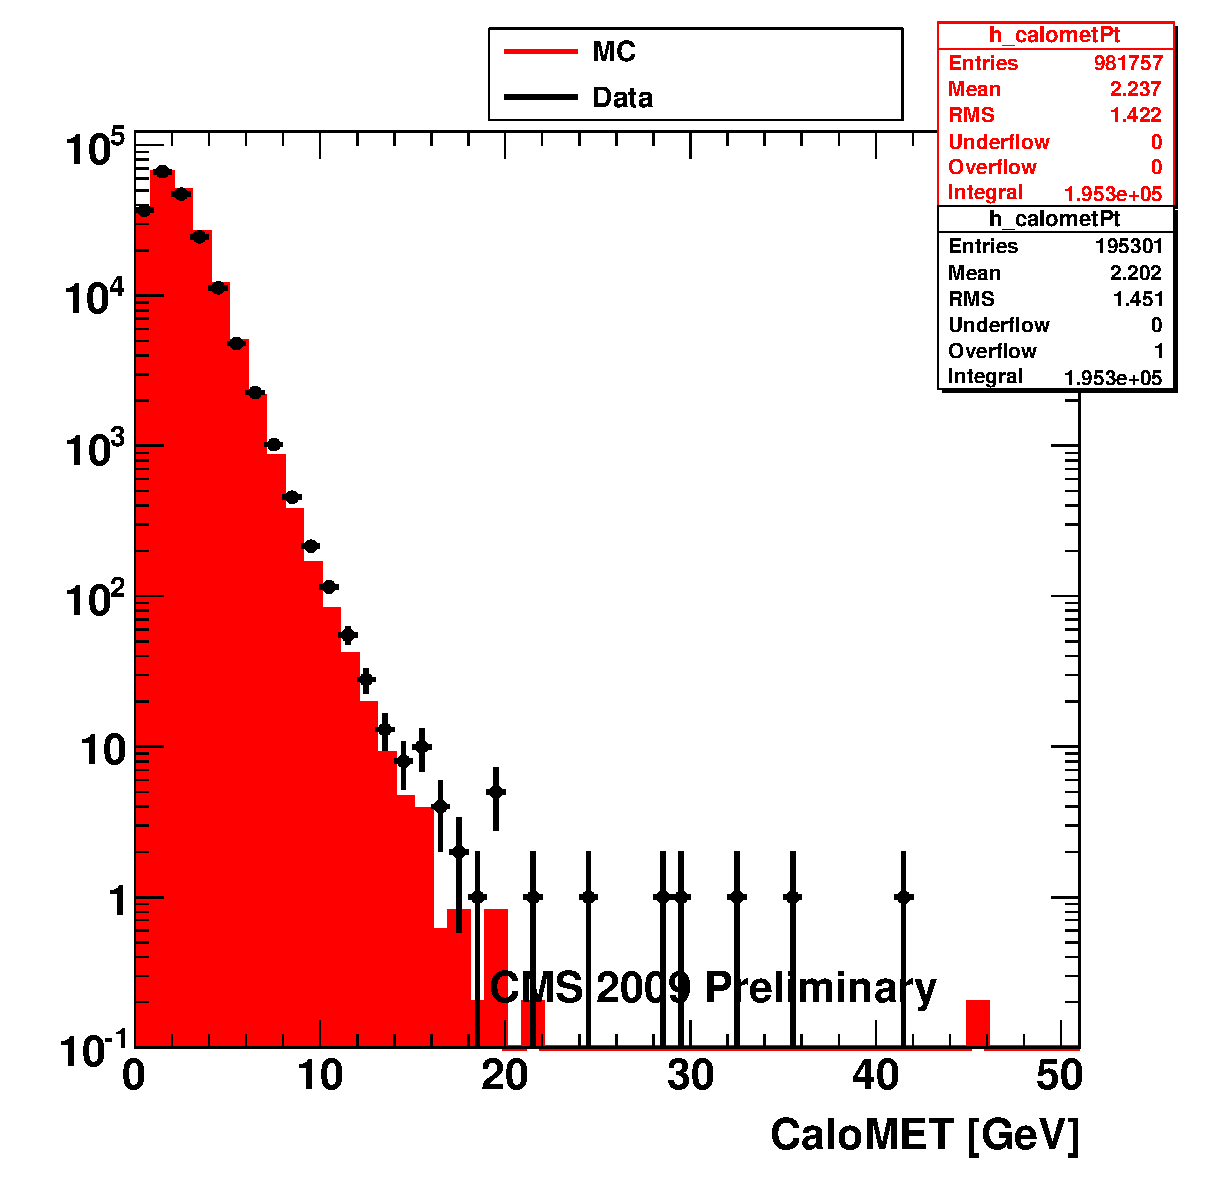
\includegraphics[width=0.40\textwidth]{plots_DataVsMC_MB_900GeV/h_calometPt.eps} &
  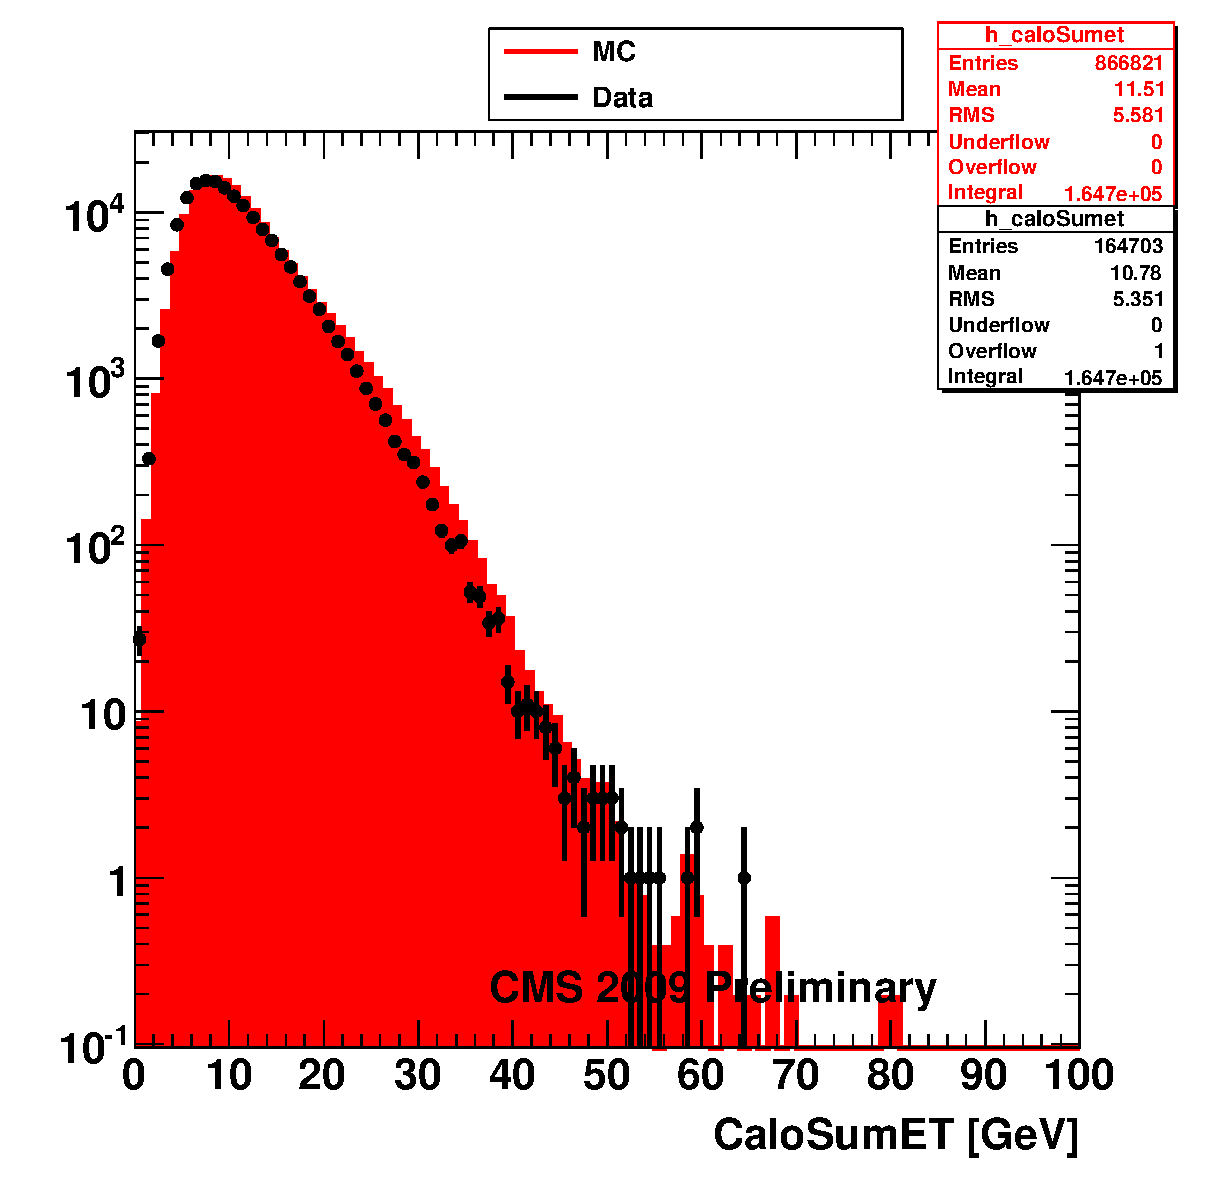
\includegraphics[width=0.40\textwidth]{plots_DataVsMC_MB_900GeV/h_caloSumet.eps} \\
 \end{tabular}
 \caption{$\etmiss$ and SumET distributions in 900 GeV data compared
   with Monte Carlo simulation.
          \label{fig:DataVsMC_MB_900_1}}
\end{figure}

\begin{figure}[h!]
 \centering
 \begin{tabular}{ll}
  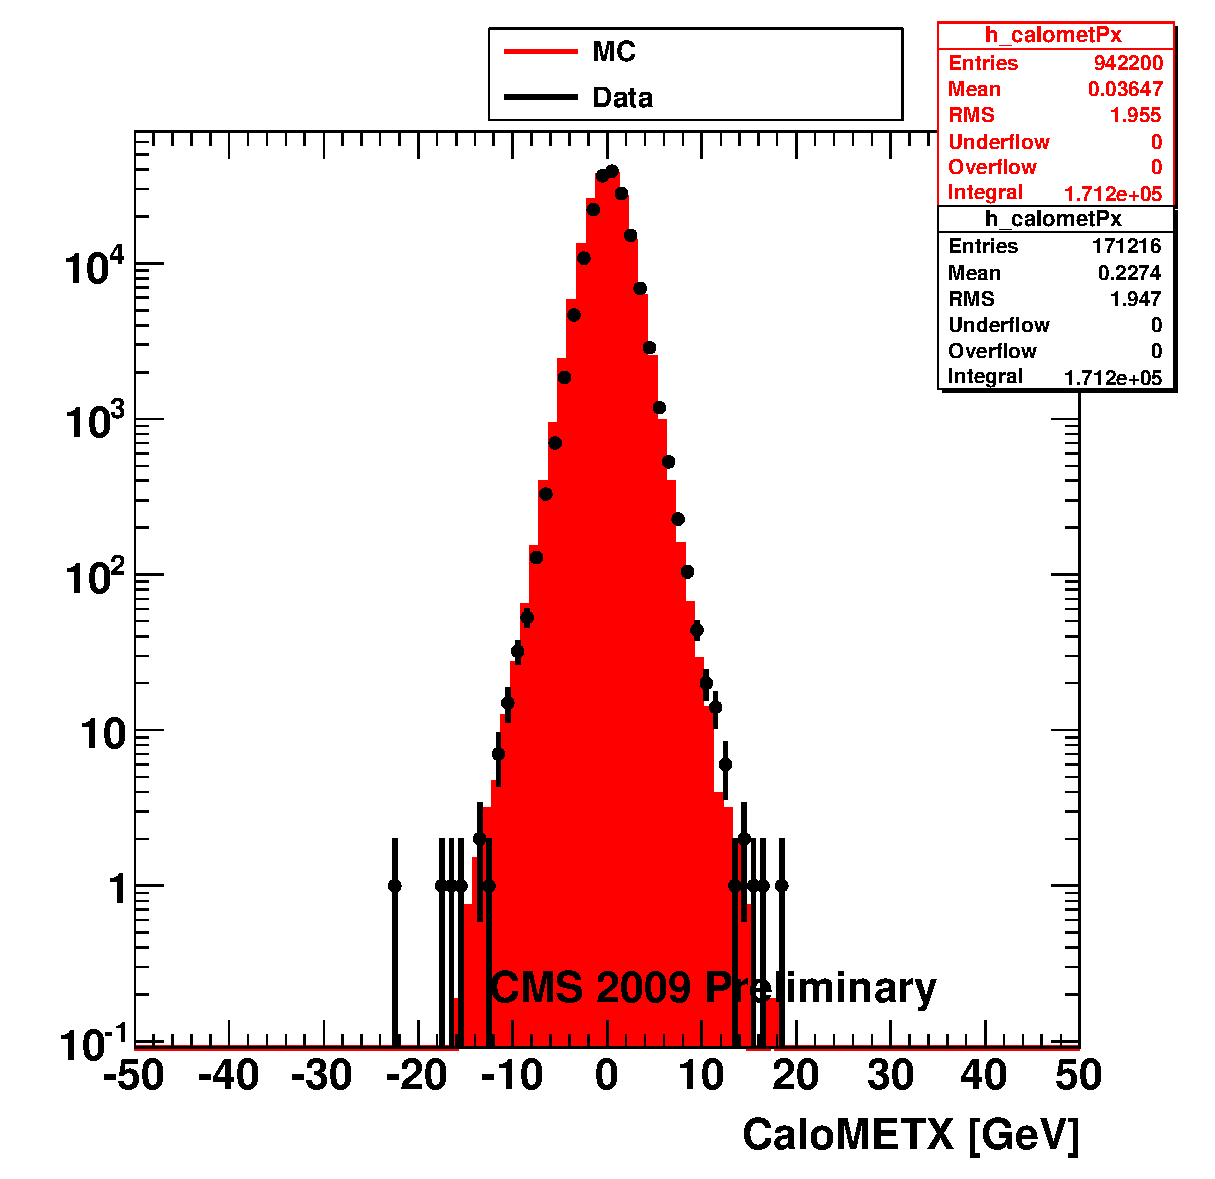
\includegraphics[width=0.40\textwidth]{plots_DataVsMC_MB_900GeV/h_calometPx.eps} &
  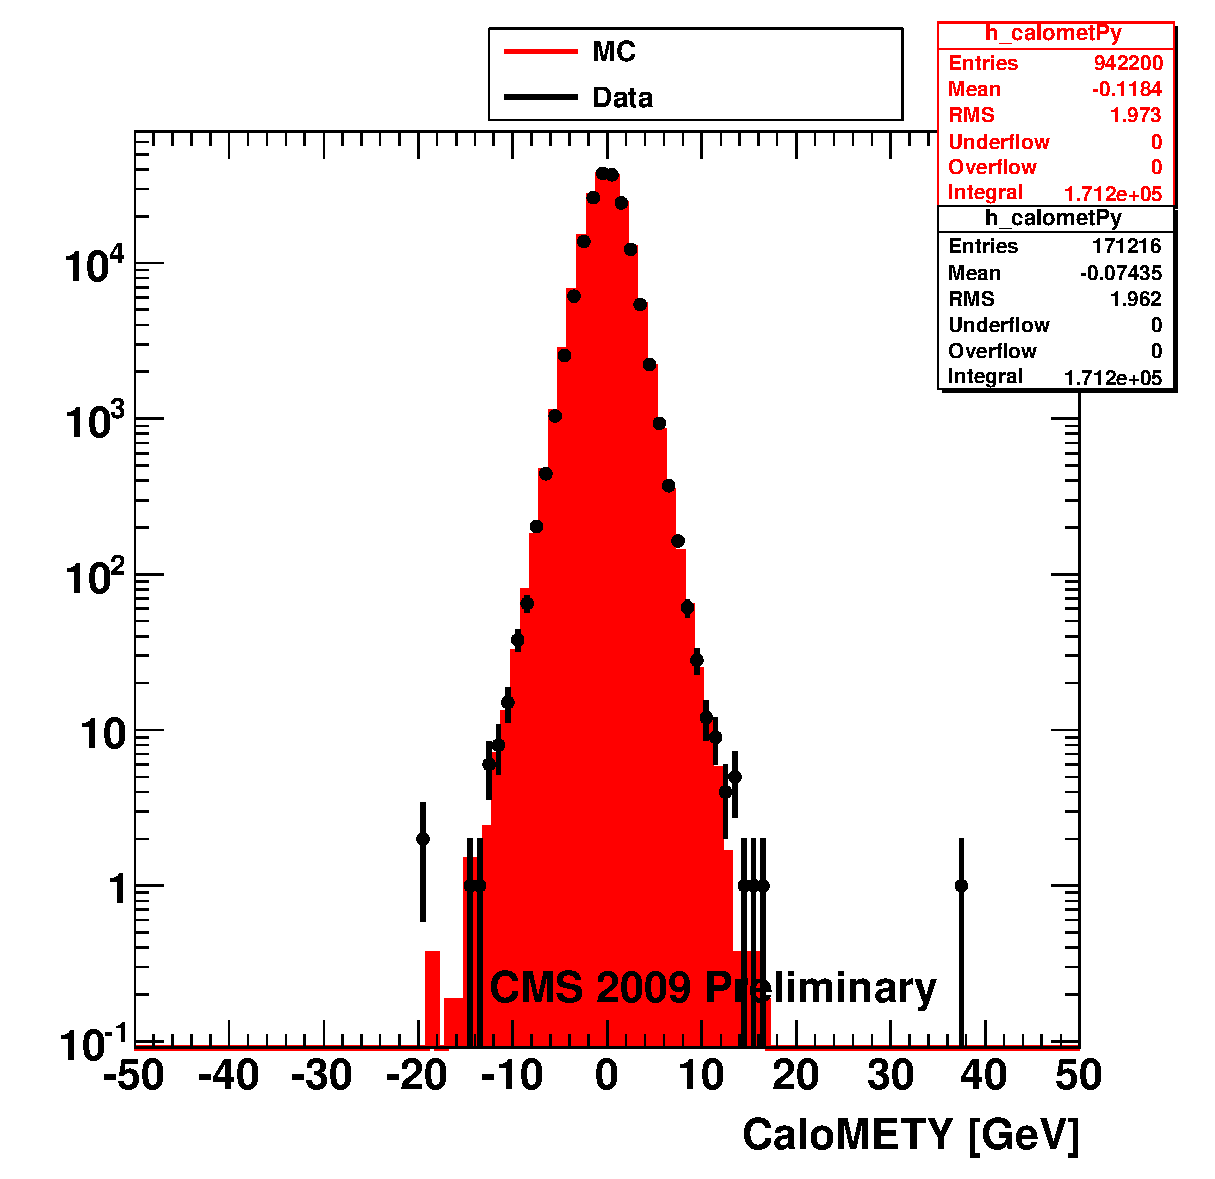
\includegraphics[width=0.40\textwidth]{plots_DataVsMC_MB_900GeV/h_calometPy.eps} \\
 \end{tabular}
 \caption{$\exmiss$ and $\eymiss$ distributions in 900 GeV data compared
   with Monte Carlo simulation.
          \label{fig:DataVsMC_MB_900_2}}
\end{figure}

\begin{figure}[h!]
 \centering
 \begin{tabular}{ll}
  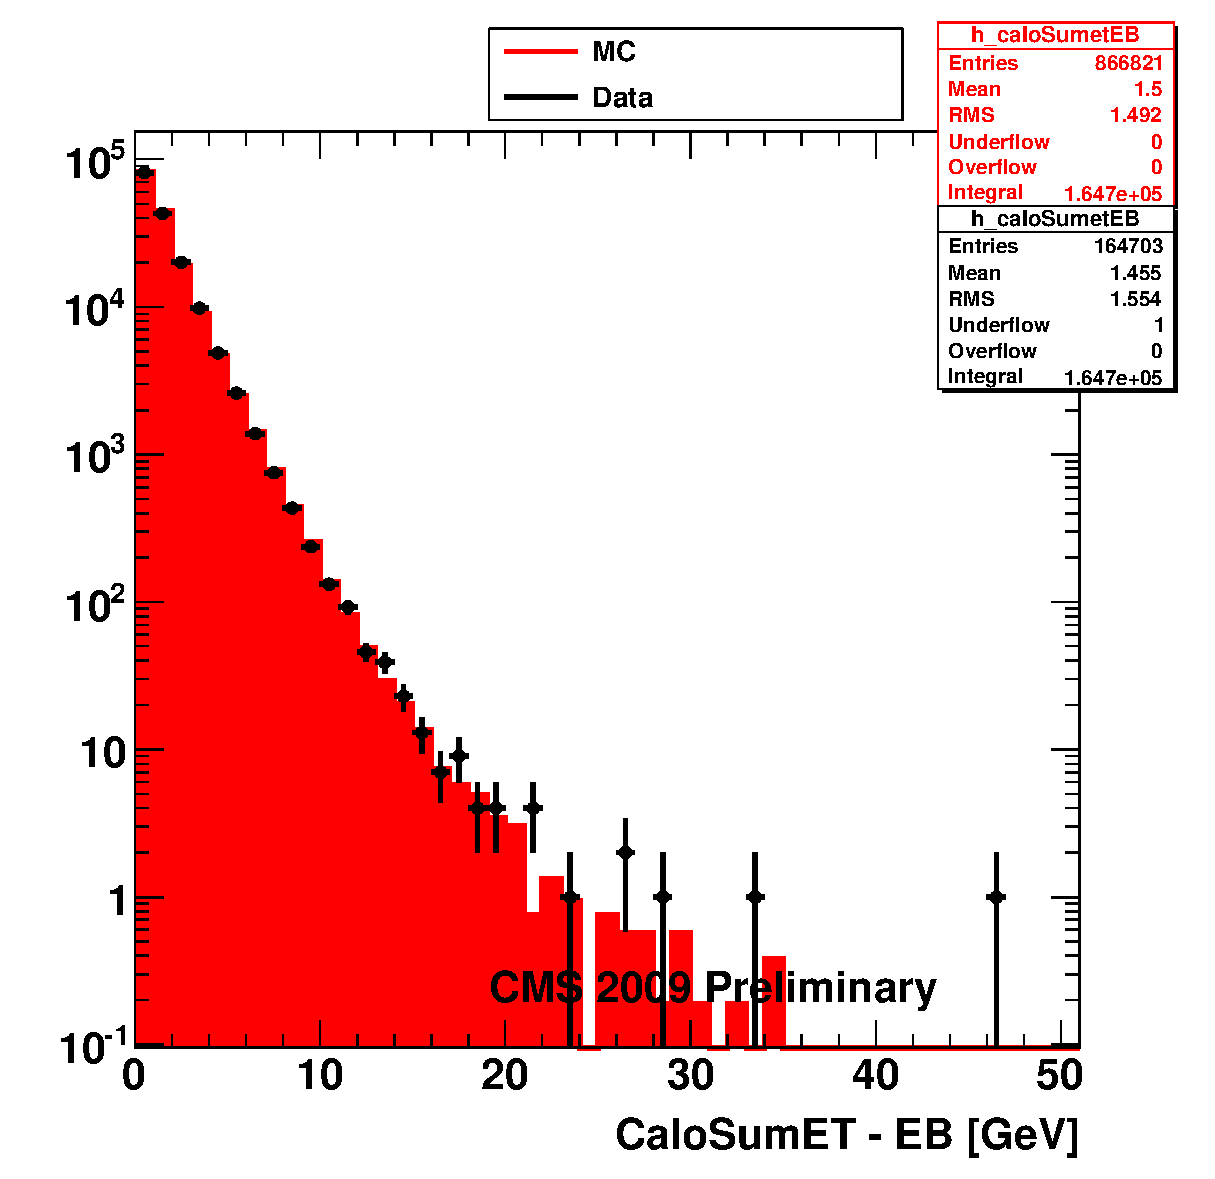
\includegraphics[width=0.40\textwidth]{plots_DataVsMC_MB_900GeV/h_caloSumetEB.eps} &
  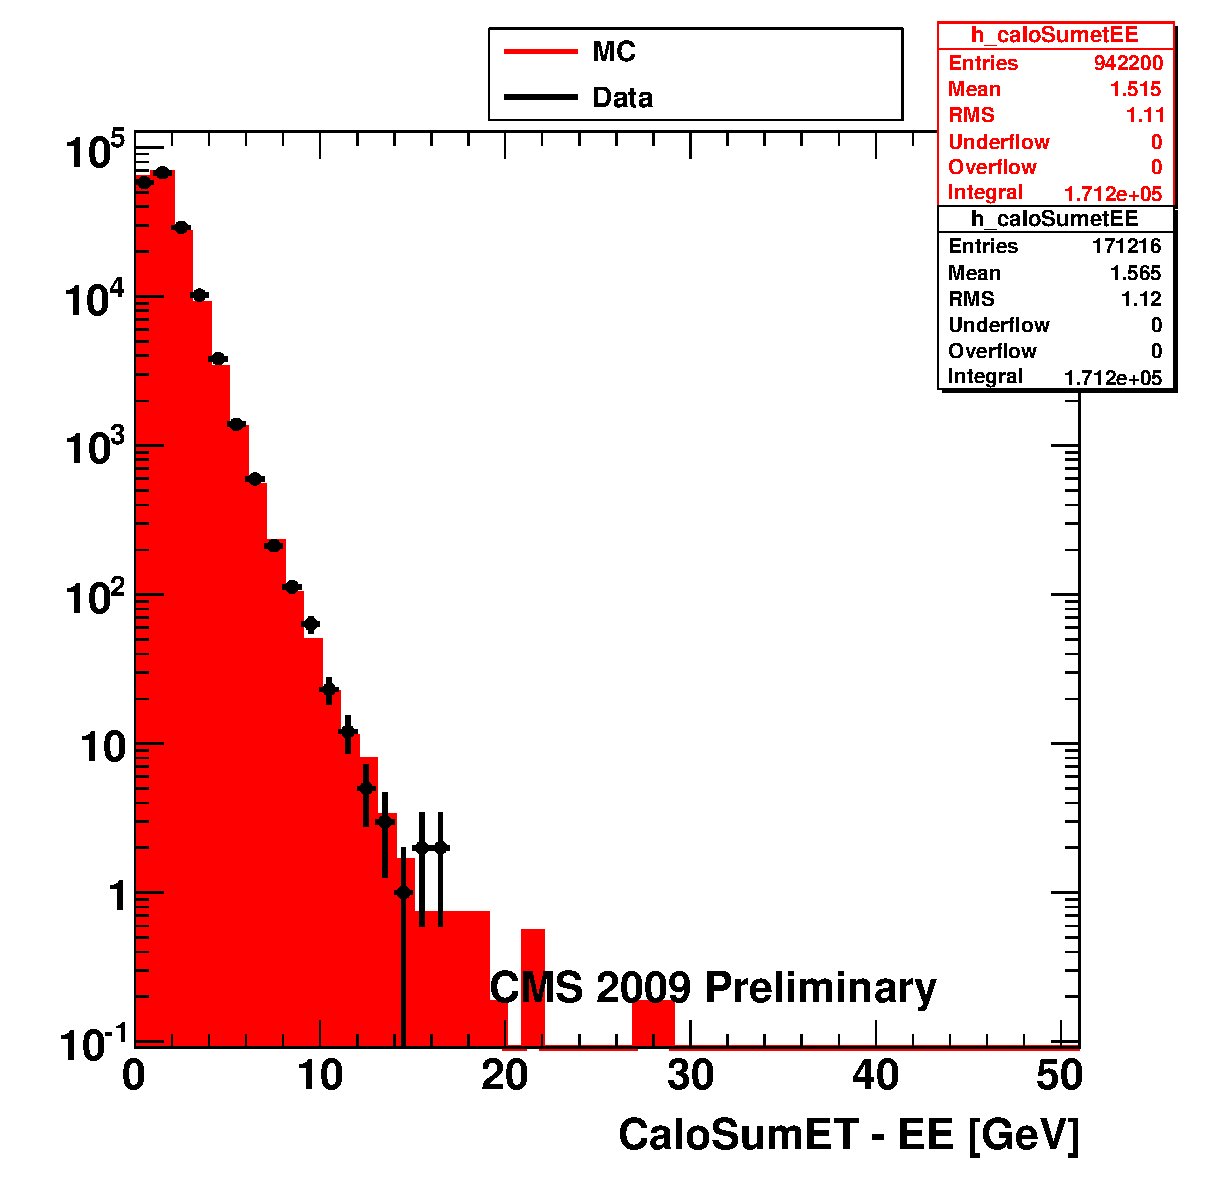
\includegraphics[width=0.40\textwidth]{plots_DataVsMC_MB_900GeV/h_caloSumetEE.eps} \\
 \end{tabular}
 \caption{SumET in ECAL barrel and endcap in 900 GeV data compared
   with Monte Carlo simulation.
          \label{fig:DataVsMC_MB_900_4}}
\end{figure}

\begin{figure}[h!]
 \centering
 \begin{tabular}{ll}
  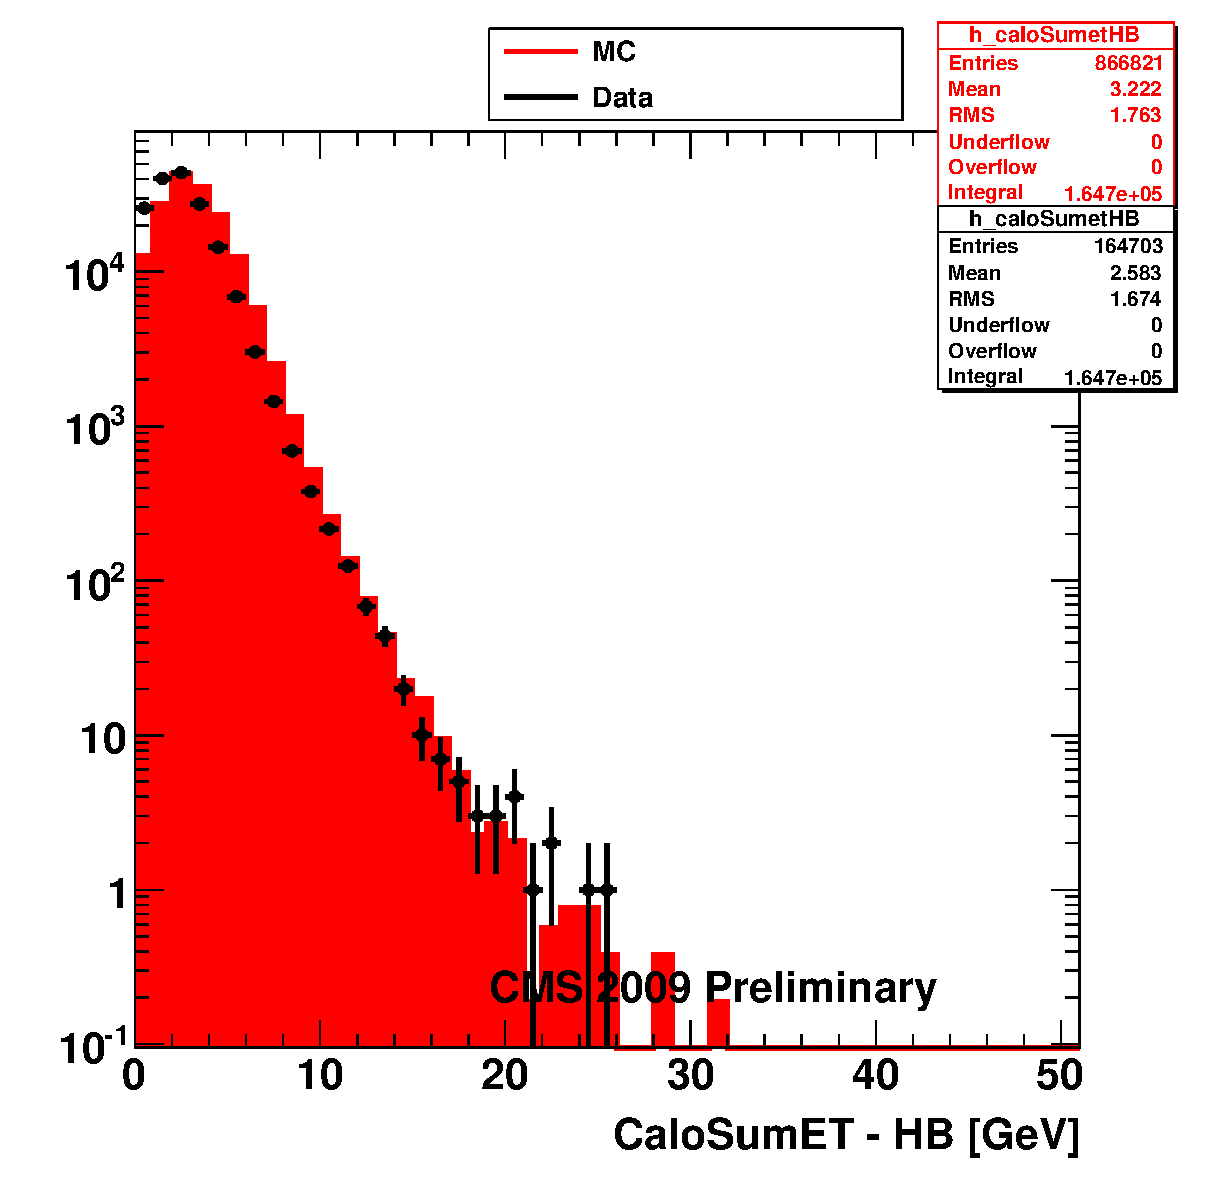
\includegraphics[width=0.40\textwidth]{plots_DataVsMC_MB_900GeV/h_caloSumetHB.eps} &
  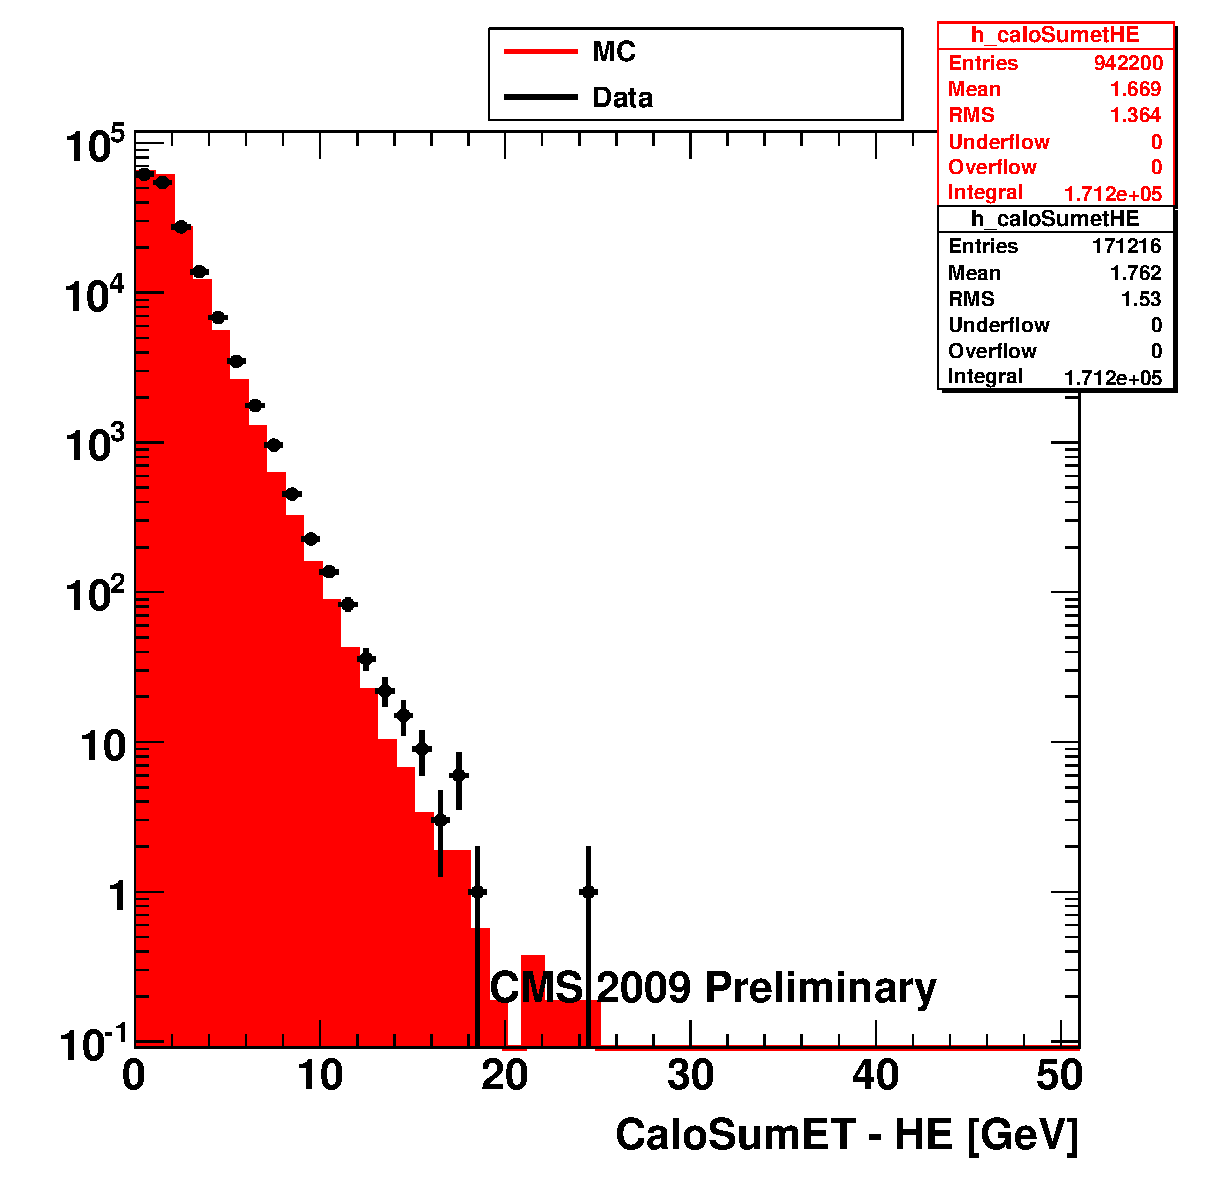
\includegraphics[width=0.40\textwidth]{plots_DataVsMC_MB_900GeV/h_caloSumetHE.eps} \\
 \end{tabular}
 \caption{SumET in HCAL barrel and endcap in 900 GeV data compared
   with Monte Carlo simulation.
          \label{fig:DataVsMC_MB_900_5}}
\end{figure}

\begin{figure}[h!]
 \centering
 \begin{tabular}{ll}
  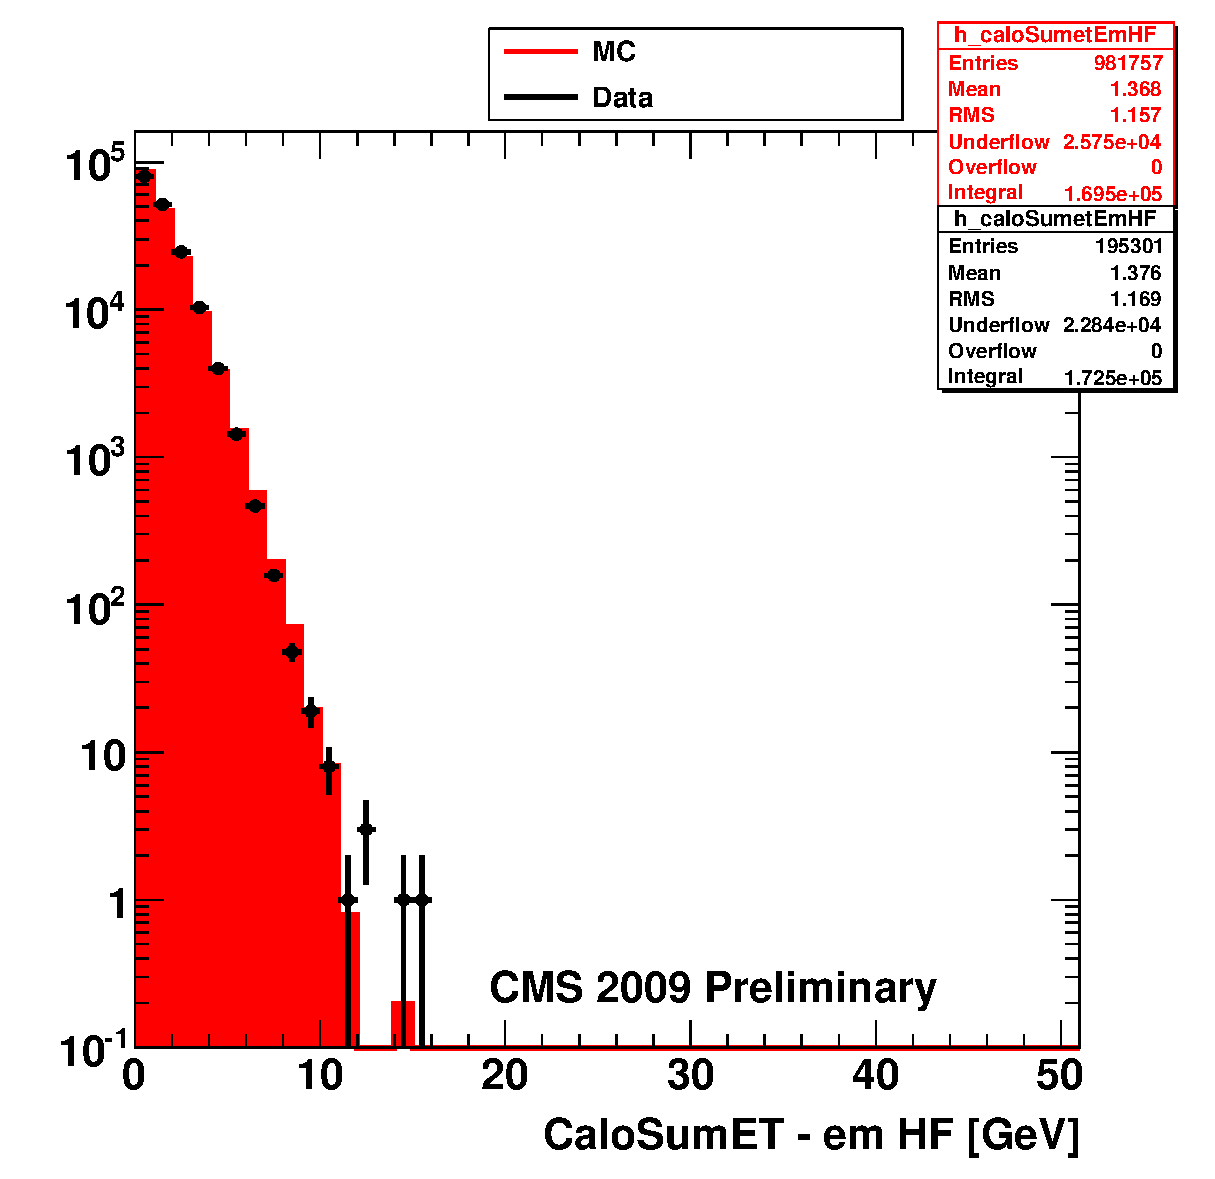
\includegraphics[width=0.40\textwidth]{plots_DataVsMC_MB_900GeV/h_caloSumetEmHF.eps} &
  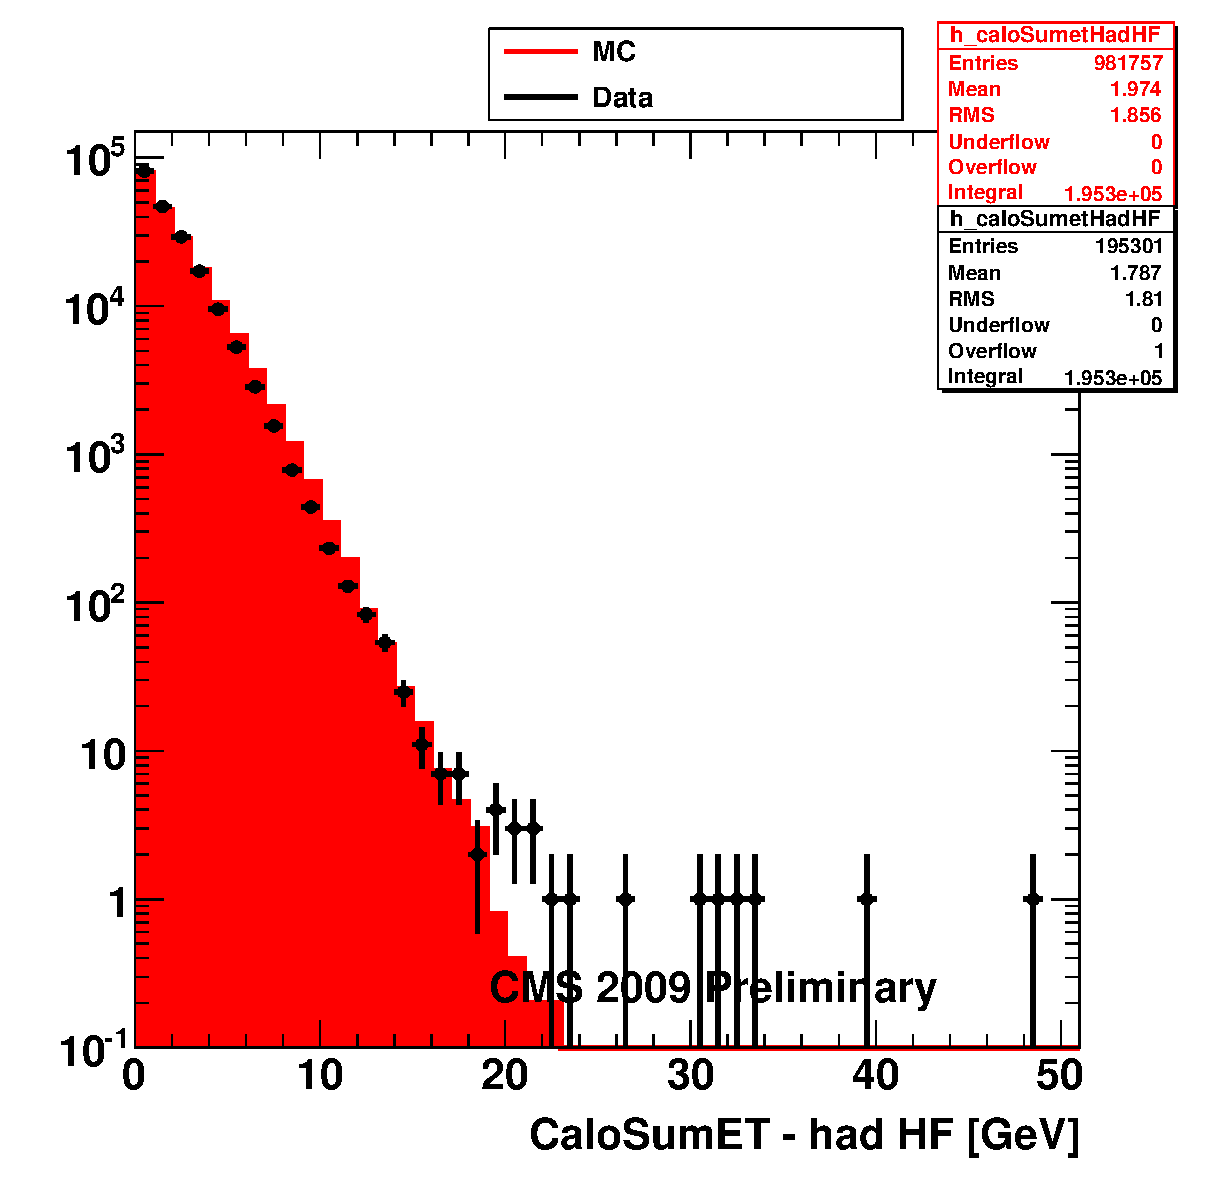
\includegraphics[width=0.40\textwidth]{plots_DataVsMC_MB_900GeV/h_caloSumetHadHF.eps} \\
 \end{tabular}
 \caption{SumET in HF in electromagnetic and hadronic parts in 900 GeV data compared
   with Monte Carlo simulation.
          \label{fig:DataVsMC_MB_900_6}}
\end{figure}

\begin{figure}[h!]
 \centering
  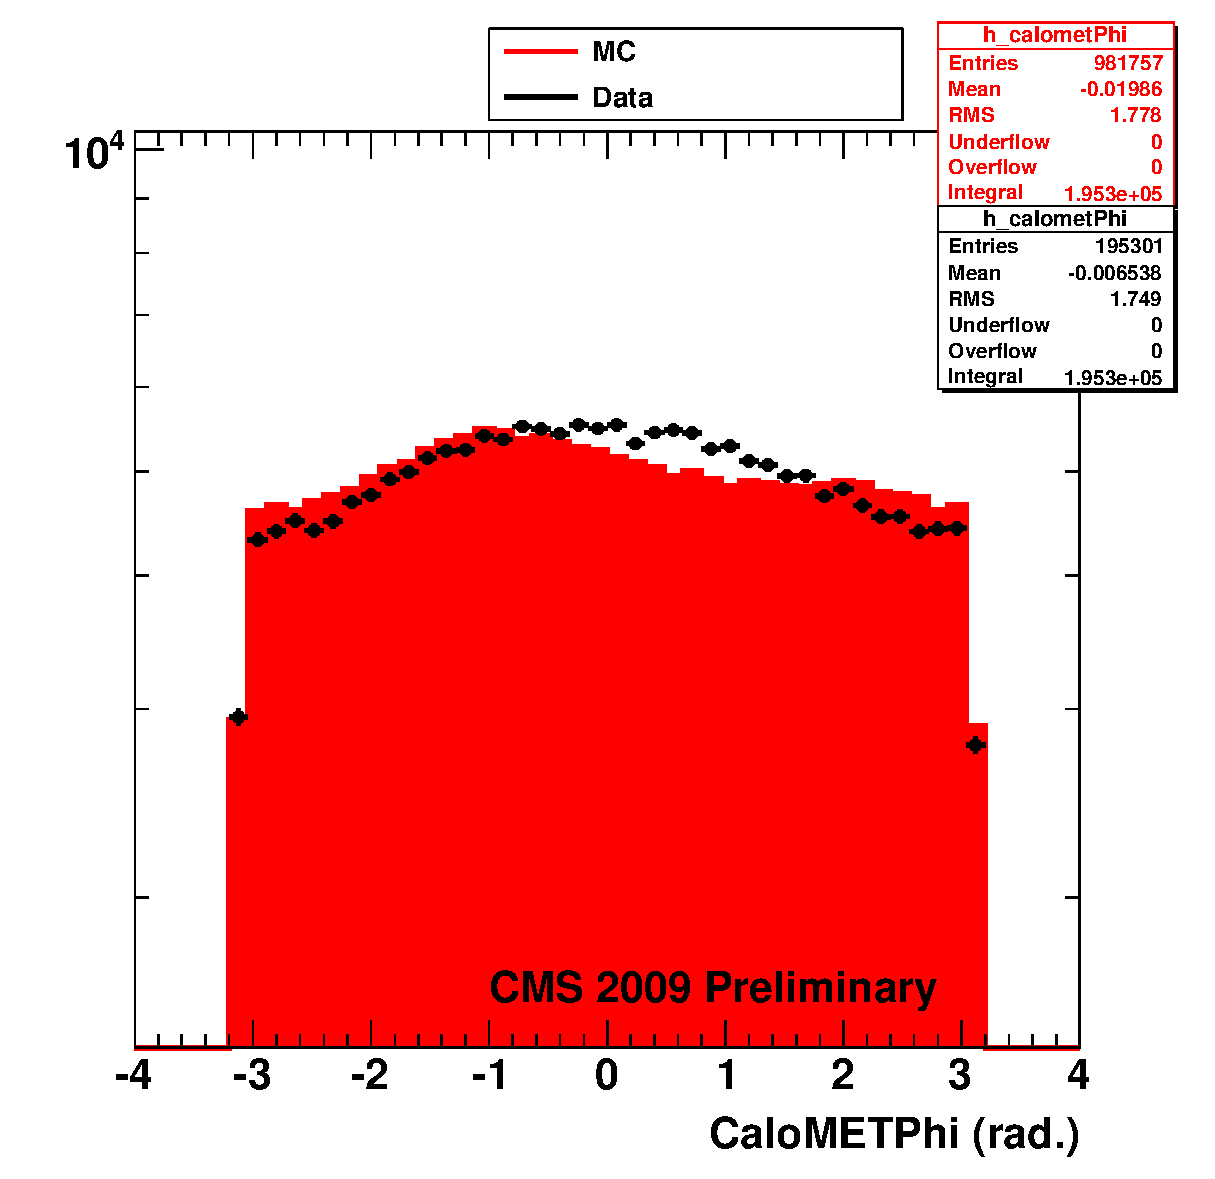
\includegraphics[width=0.40\textwidth]{plots_DataVsMC_MB_900GeV/h_calometPhi.eps}
 \caption{$\phi_{\etmiss}$ distributions in 900 GeV data compared
   with Monte Carlo simulation.
          \label{fig:DataVsMC_MB_900_7}}
\end{figure}

\begin{figure}[h!]
 \centering
 \begin{tabular}{ll}
  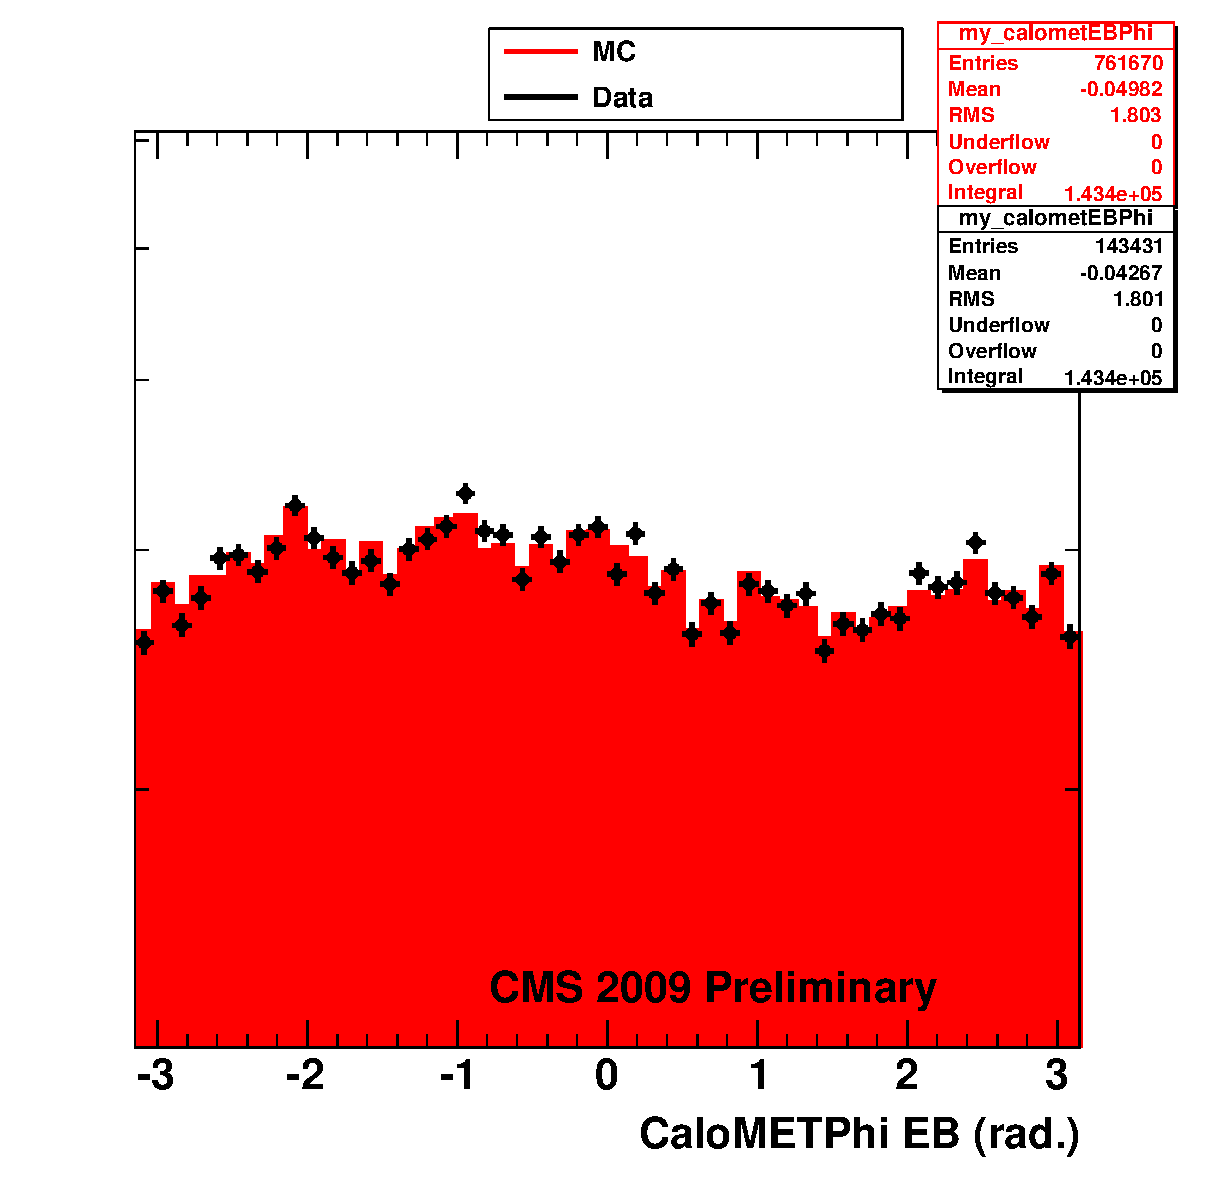
\includegraphics[width=0.40\textwidth]{plots_DataVsMC_MB_900GeV/my_calometEBPhi.eps} &
  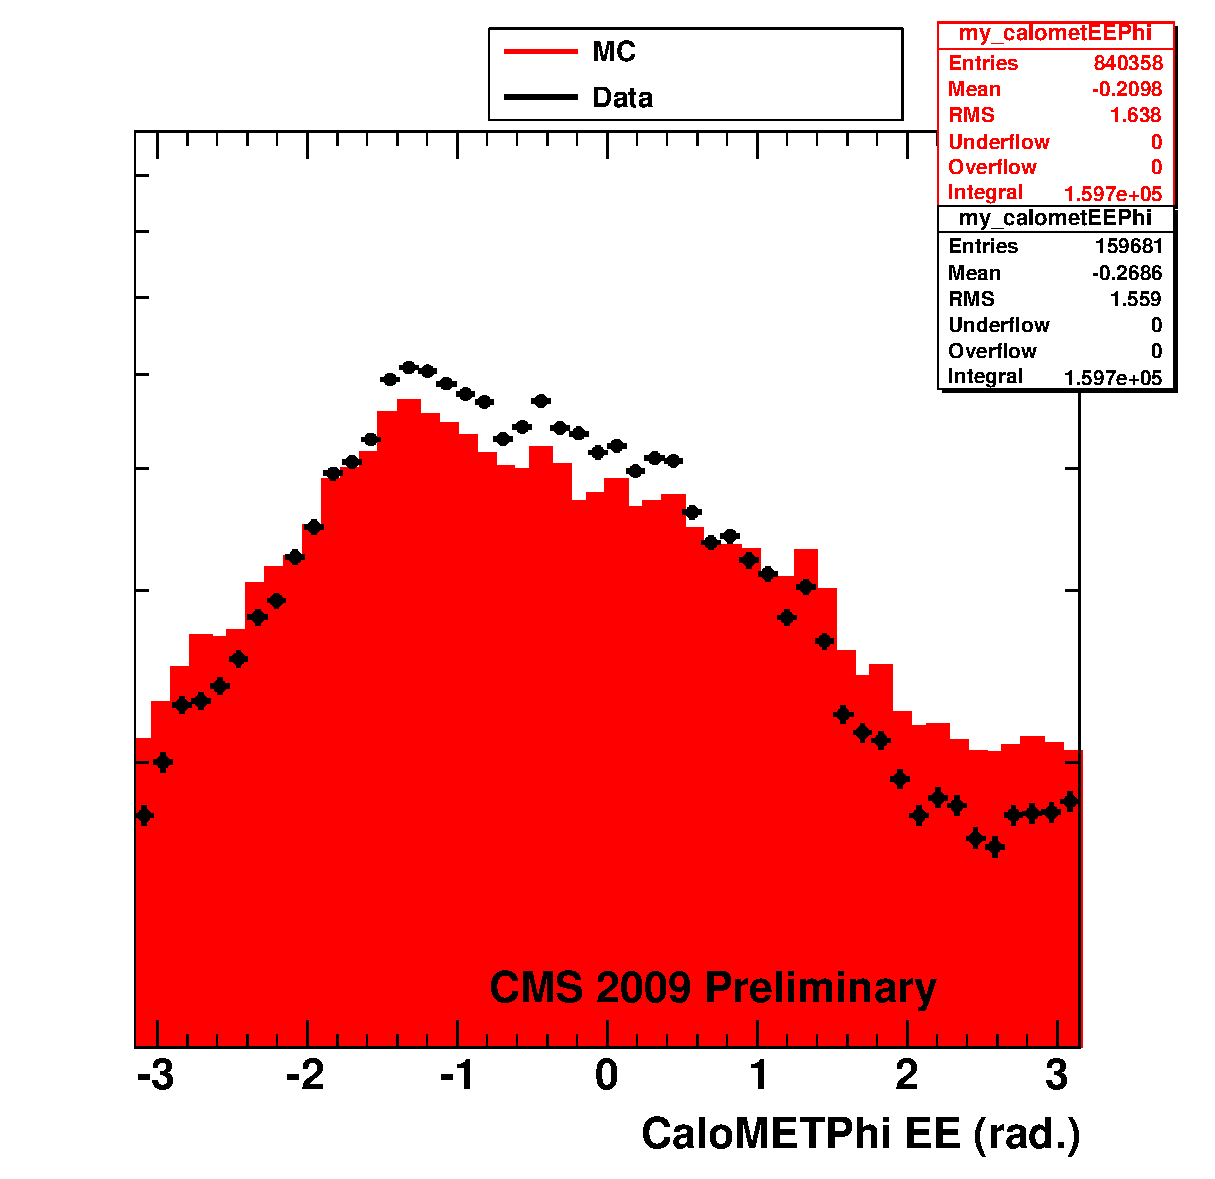
\includegraphics[width=0.40\textwidth]{plots_DataVsMC_MB_900GeV/my_calometEEPhi.eps} \\
 \end{tabular}
 \caption{$\phi_{\etmiss}$ distributions in ECAL barrel and endcap in 900 GeV data compared
   with Monte Carlo simulation.
          \label{fig:DataVsMC_MB_900_8}}
\end{figure}

\begin{figure}[h!]
 \centering
 \begin{tabular}{ll}
  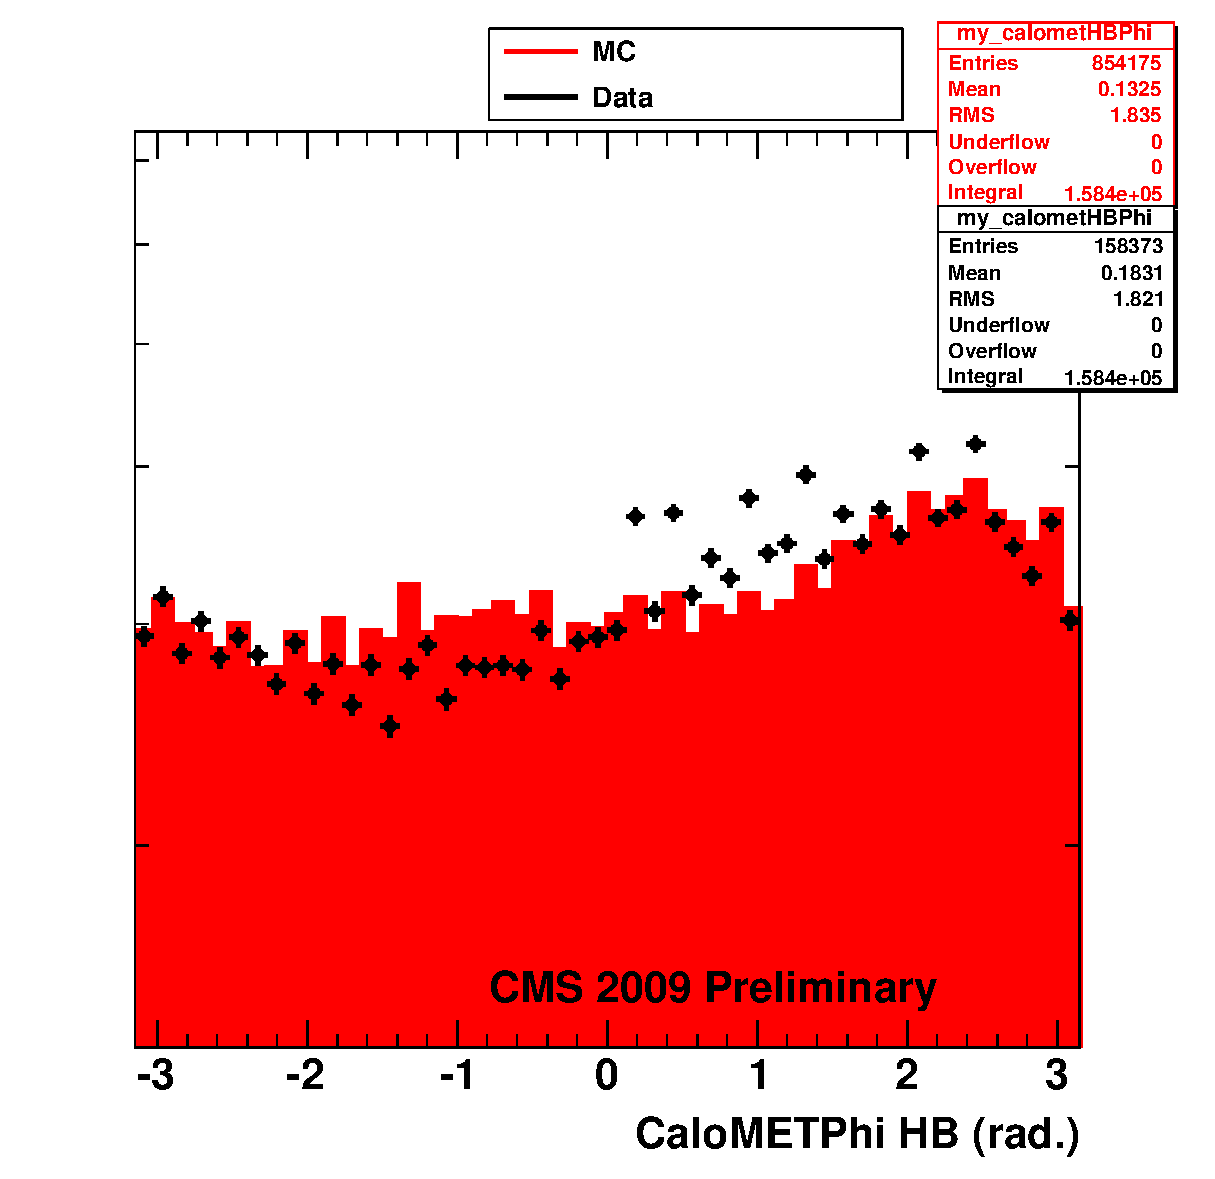
\includegraphics[width=0.40\textwidth]{plots_DataVsMC_MB_900GeV/my_calometHBPhi.eps} &
  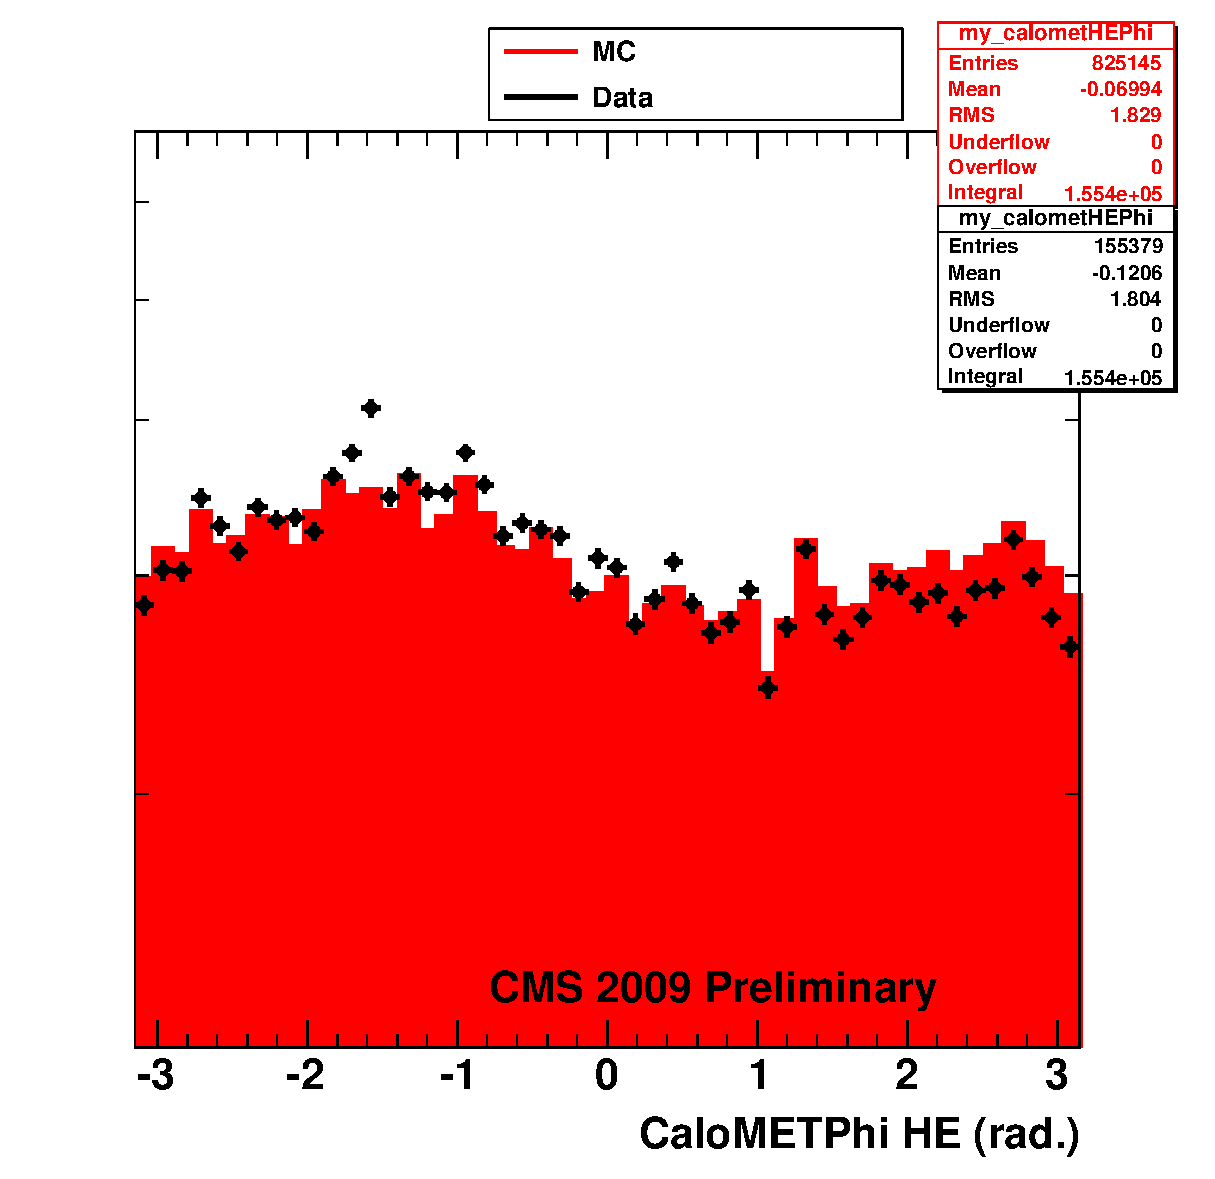
\includegraphics[width=0.40\textwidth]{plots_DataVsMC_MB_900GeV/my_calometHEPhi.eps} \\
 \end{tabular}
 \caption{$\phi_{\etmiss}$ distributions in HCAL barrel and endcap in 900 GeV data compared
   with Monte Carlo simulation.
          \label{fig:DataVsMC_MB_900_9}}
\end{figure}

\begin{figure}[h!]
 \centering
 \begin{tabular}{ll}
  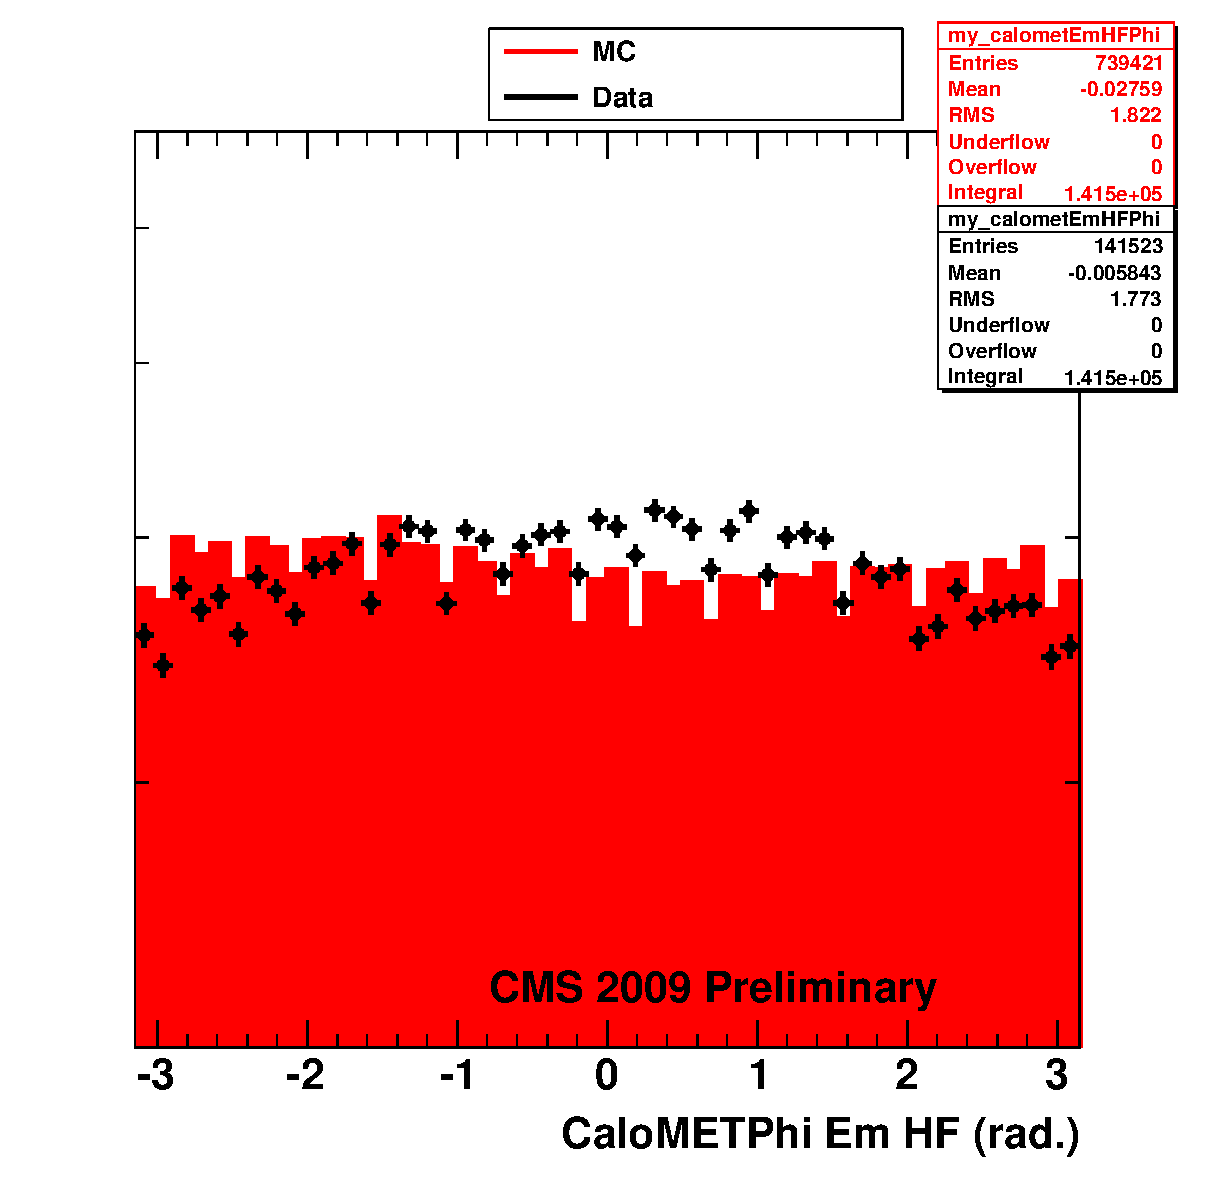
\includegraphics[width=0.40\textwidth]{plots_DataVsMC_MB_900GeV/my_calometEmHFPhi.eps} &
  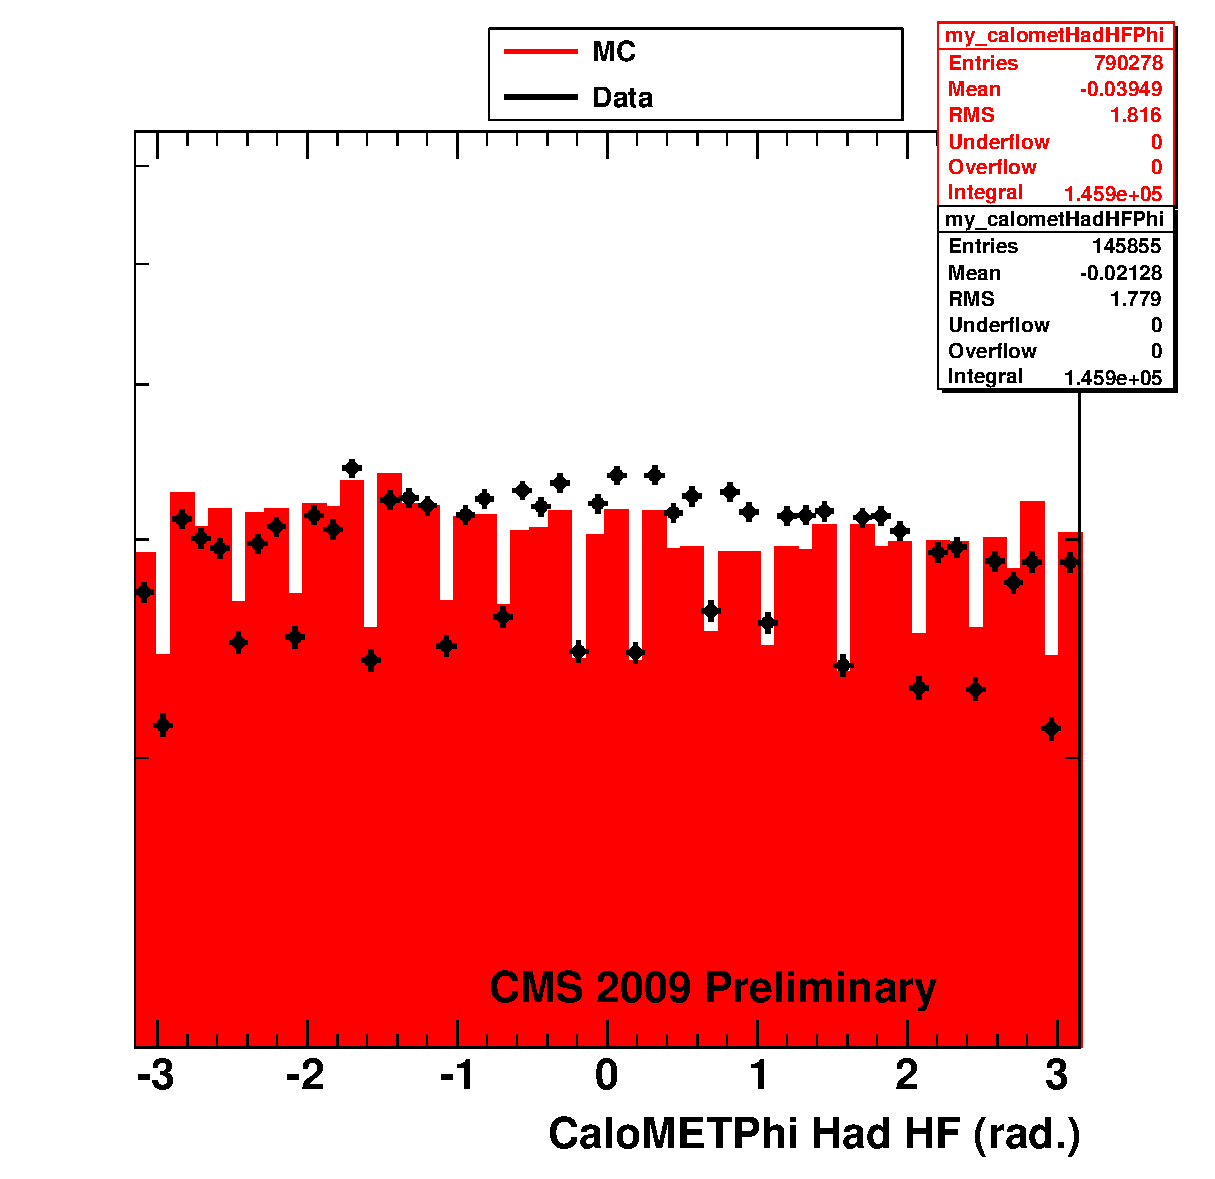
\includegraphics[width=0.40\textwidth]{plots_DataVsMC_MB_900GeV/my_calometHadHFPhi.eps} \\
 \end{tabular}
 \caption{$\phi_{\etmiss}$ distributions in HF in electromagnetic and hadronic parts in 900 GeV data compared
   with Monte Carlo simulation.
          \label{fig:DataVsMC_MB_900_10}}
\end{figure}


Some of the features of the $\etmiss>15$~GeV events are listed below,
ordered by decreasing values of reconstructed $\etmiss$:
\begin{itemize}
\item $\etmiss=40.7752$~GeV, $\exmiss=-17.1$~GeV, $\eymiss=37.0$~GeV:
  Run 124024, ls 52, event 19351796: Two energetic HF towers are present
  in the event, close to each other in the same $\phi$. For one of the
  towers $E_{T}(L)=1.65308$~GeV, $E_{T}(S)=10.2048$~GeV and for the
  second one $E_{T}(L)=19.8857$~GeV, $E_{T}(S)=12.6117$~GeV. The event
  does not look like a HF PMT hit, however there is very little energy
  deposited in the neighbourhood of the two towers above.

\item $\etmiss=24.7444$~GeV, $\exmiss=-22.1$~GeV, $\eymiss=-11.2$~GeV:
  Run 124020, ls 57, event: 20853863: two neighbouring towers in HCAL,
  probably HPD noise. No energy deposit in ECAL.

\item $\etmiss=21.6884$~GeV, $\exmiss=9.6$~GeV, $\eymiss=-19.4$~GeV: Run
  124027, ls 35, event 12262783: an energetic tower in HF,
  $E_{T}(L)=16.3871$~GeV,
  $E_{T}(S)=0.215171$~GeV. $(L-S)/(L+S)=0.97$. Could be a PMT hit.

\item $\etmiss=19.9143$~GeV, $\exmiss=-11.8$~GeV, $\eymiss=16.0$~GeV:
  Run 124024, ls 78, event 28980731: not clear, looks like a real energy
  deposit in a few neihboring HF towers.

\item $\etmiss=19.6766$~GeV, $\exmiss=2.8$~GeV, $\eymiss=-19.5$~GeV: Run
  124030, ls 8, event 2665873: an energetic tower in HF, $E_{T}(L)=
  13.5777$~GeV, $E_{T}(S)=0.517116$~GeV. $(L-S)/(L+S)=0.93$. Small
  energy deposits in the neighbouring towers, could be a physics event
  with the unbalanced energy lost down the beam pipe.

\item $\etmiss=19.5558 $~GeV: Run 124023, ls 46, event 5522301: three
  neighbouring towers in HB, could be an HPD noise. No energy in ECAL

\item $\etmiss=18.5625$~GeV, $\exmiss=18.5$~GeV, $\eymiss=1.4$~GeV: Run
  124030, ls 14, event 4893420: there are 4 jets in the event, which are
  back-to-back and one is undermeasured.

\item $\etmiss=18.1722$~GeV: Run 124020, ls 35, event 12386199:
  undermeasured energy, many soft deposits here and there.

\item $\etmiss=17.3232$~GeV, $\exmiss=16.7$~GeV, $\eymiss=-4.5$~GeV: Run
  124023, ls 50, event 6957103: 3 neihboring HB towers, no ECAL
  deposits, likely HPD noise.

\item $\etmiss=16.8036$~GeV, $\exmiss=-16.6$~GeV, $\eymiss=2.5$~GeV: Run
  124024, ls 80, event 29768956: several neighbouring towers in HF,
  unlikely to be a PMT hit, maybe unbalanced energy left down the beam
  pipe.

\item $\etmiss=16.3845$~GeV: Run 124023, ls 65, event 12466348: a single
  energetic tower in HF, $E_{T}(L)= 11.3415$~GeV,
  $E_{T}(S)=0.4685$~GeV. $(L-S)/(L+S)=0.92$. May be a PMT hit.

\item $\etmiss=16.2618$~GeV: Run 124023, ls 50, event 7040081: a few
  neihboring towers in HF, does not look like a PMT hit.

\item $\etmiss=15.5162$~GeV, $\exmiss=-15.0$~GeV, $\eymiss=-3.9$~GeV:
  Run 124025, ls 7, event 2194922: a few neighbouring towers in HF,
  unlikely to be a PMT hit.

\item $\etmiss=15.4445$~GeV: Run 124027, ls 26, event 8792680: a few
  neighbouring towers in HB, but not same phi. Maybe unbalanced energy
  went down the beam pipe.

\item $\etmiss=15.8119$~GeV, $\exmiss=15.8$~GeV, $\eymiss=-0.3$~GeV: Run
  124024, ls 21, event 7735977: two neihboring towers in HB, same
  $\eta$.  No energy deposits in ECAL at the same location, maybe HB
  noise.

\item $\etmiss=15.2424$~GeV, $\exmiss=-0.1$~GeV, $\eymiss=-15.2$~GeV:
  Run 124022, ls 130, event 29704007: a tower in HB with $E_T\sim 8$~GeV
  with a few neihbors, no ECAL deposit.
\end{itemize}


\begin{figure}[h!]
  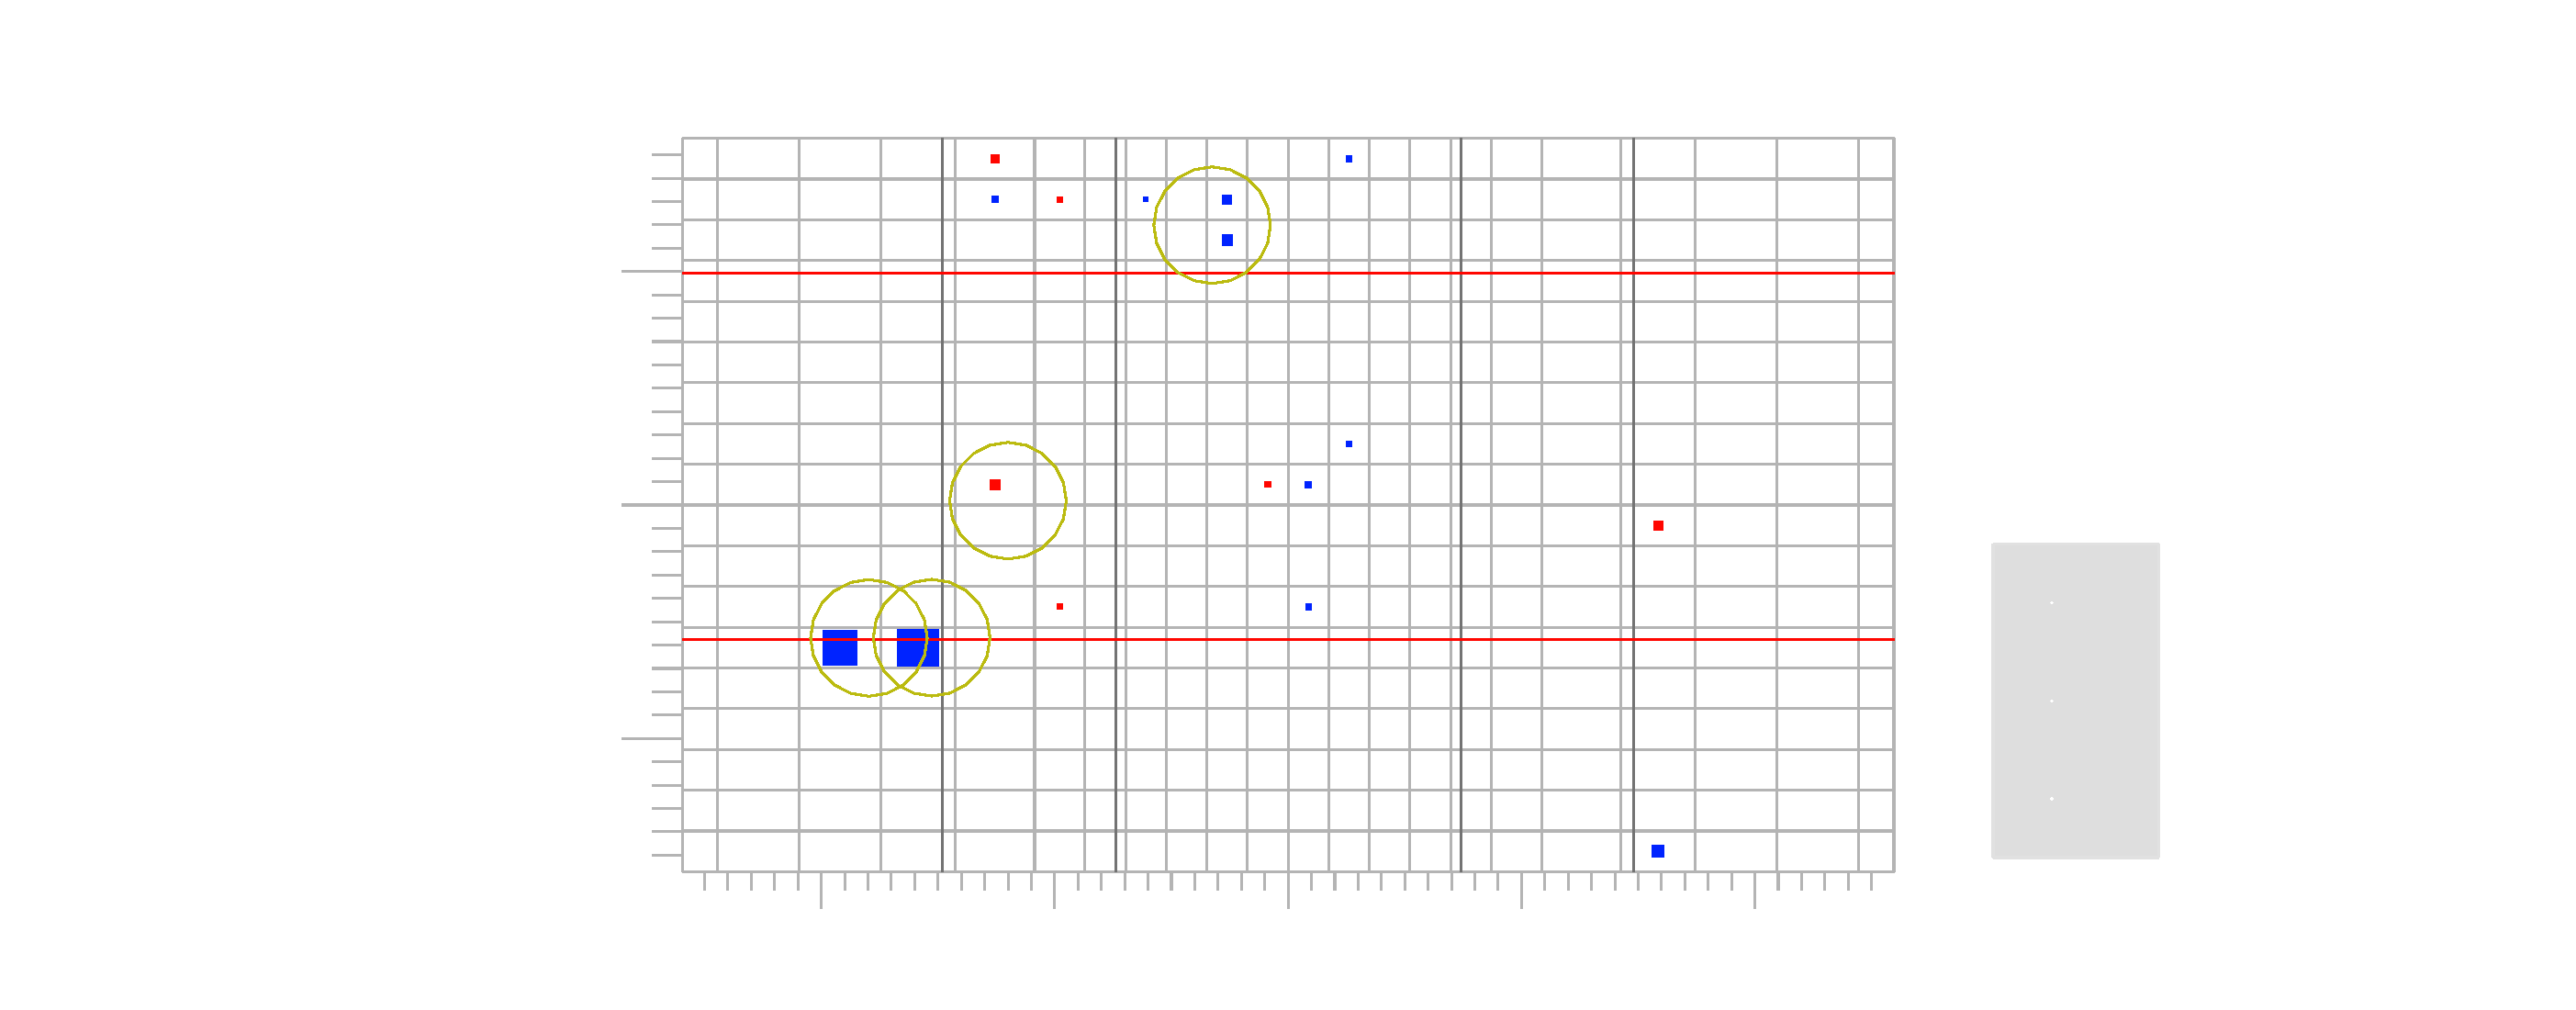
\includegraphics[width=12cm]{plots_DataVsMC_MB_900GeV/124024_19351796_MET41GeV.eps}
  \caption{Lego plot of the highest $\etmiss=41.04$~GeV event (Run 124024, ls 52, event 19351796). It appears
    that the $\etmiss$ is caused by an HF PMT hit.
    \label{fig:DataVsMC_MB_900_evd1}}
\end{figure}

\begin{figure}[h!]
  \includegraphics[width=12cm]{plots_DataVsMC_MB_900GeV/124030_4893420_4jet.eps}
  \caption{The $\etmiss=19.987$~GeV event (Run 124030, ls
    14, event 4893420). This event seems to contain 4 jets, one of which
    is severly undermeasured causing the $\etmiss$.
    \label{fig:DataVsMC_MB_900_evd3}}
\end{figure}


\clearpage

\subsection{$\etmiss$ resolution}

For events with no $\etmiss$ from physics sources, the $\etmiss$ resolution can be most generally parameterized
according to the following expression~\cite{CMS:AN_2007_041}:
\begin{equation}
  \sigma\left(\etmiss\right)=A \oplus B\sqrt{\sum E_\text{T}-D} \oplus C\left(\sum E_\text{T}-D\right),
  \label{eq:MET_sigma}
\end{equation}
where $A$ is the noise term, $B$ is the stohastic term, $C$ is the constant term, and $D$ is the offset term. In such events
$\exmiss$ and $\eymiss$ are expected to follow a Gaussian distribution with the mean of zero and the standard deviation
of $\sigma$. It can also be shown that $\sigma\left(\etmiss\right)$ is proportional to this $\sigma$. Therefore,
by looking at $\sigma\left(\exmiss\right)$ and $\sigma\left(\eymiss\right)$ as a function of $\sum E_\text{T}$ it is possible to
study the $\etmiss$ resolution and the relative contributions of different resolution terms at different values of $\sum E_\text{T}$.

Figure~\ref{fig:MExySigma_vs_SumET_900} shows the $\sigma\left(\exmiss\right)$ and $\sigma\left(\eymiss\right)$ 
vs. $\sum E_\text{T}$ for 900 GeV data compared with Monte Carlo simulation. $\sigma\left(\exmiss\right)$ and $\sigma\left(\eymiss\right)$
were extracted from a Gaussian fit to $\exmiss$ and $\eymiss$ distributions, respectively, in a region of $\pm 1.5$ RMS around the mean.
Figures~\ref{fig:MExSigma_vs_SumET_900_fit} and \ref{fig:MEySigma_vs_SumET_900_fit} show the fit results 
of $\sigma\left(\exmiss\right)$ and $\sigma\left(\eymiss\right)$ vs. $\sum E_\text{T}$ to Eq.~\ref{eq:MET_sigma} 
for data and Monte Carlo at $900$ GeV.

\begin{figure}[h!]
 \centering
 \begin{tabular}{ll}
  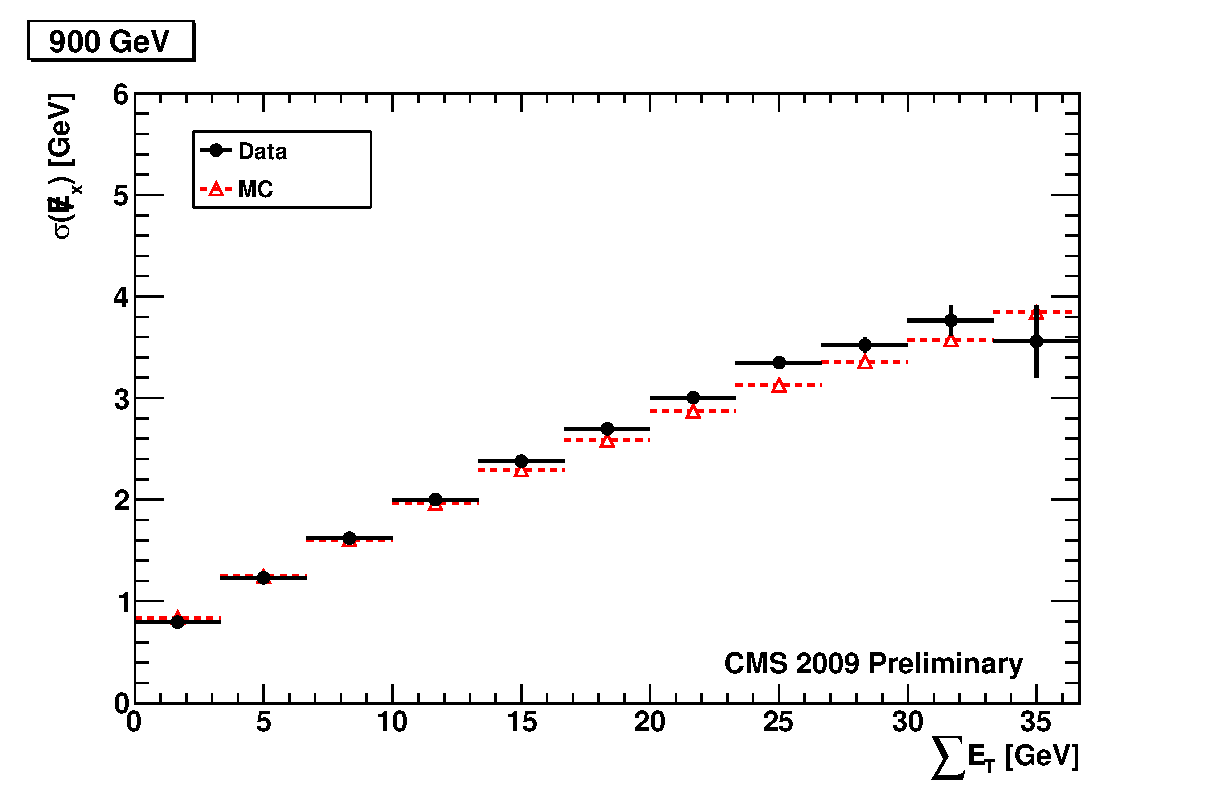
\includegraphics[width=0.5\textwidth]{plots_DataVsMC_MB_900GeV/h_metxsigma_sumet_900.eps} &
  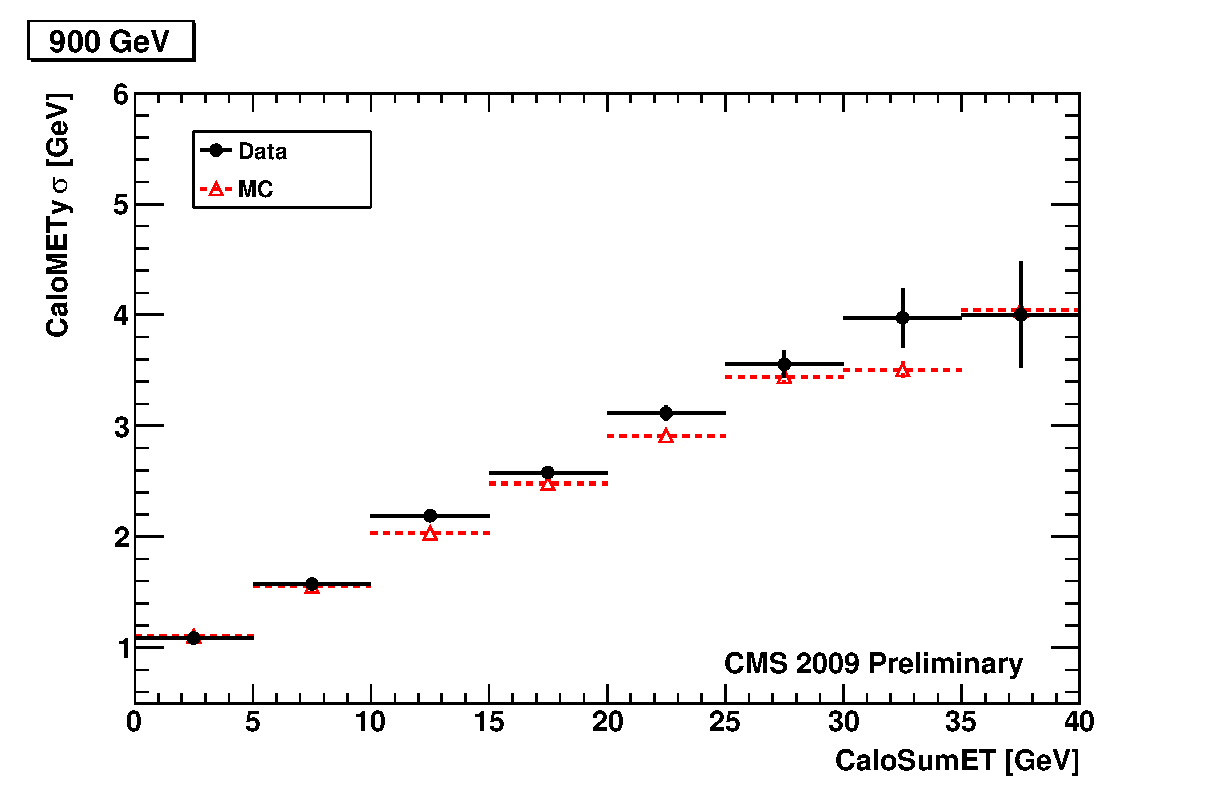
\includegraphics[width=0.5\textwidth]{plots_DataVsMC_MB_900GeV/h_metysigma_sumet_900.eps} \\
 \end{tabular}
 \caption{\small $\sigma\left(\exmiss\right)$ and $\sigma\left(\eymiss\right)$ vs. $\sum E_\text{T}$ for data at $900$ GeV
          compared with Monte Carlo simulation.\label{fig:MExySigma_vs_SumET_900}}
\end{figure}

\begin{figure}[h!]
 \centering
 \begin{tabular}{ll}
  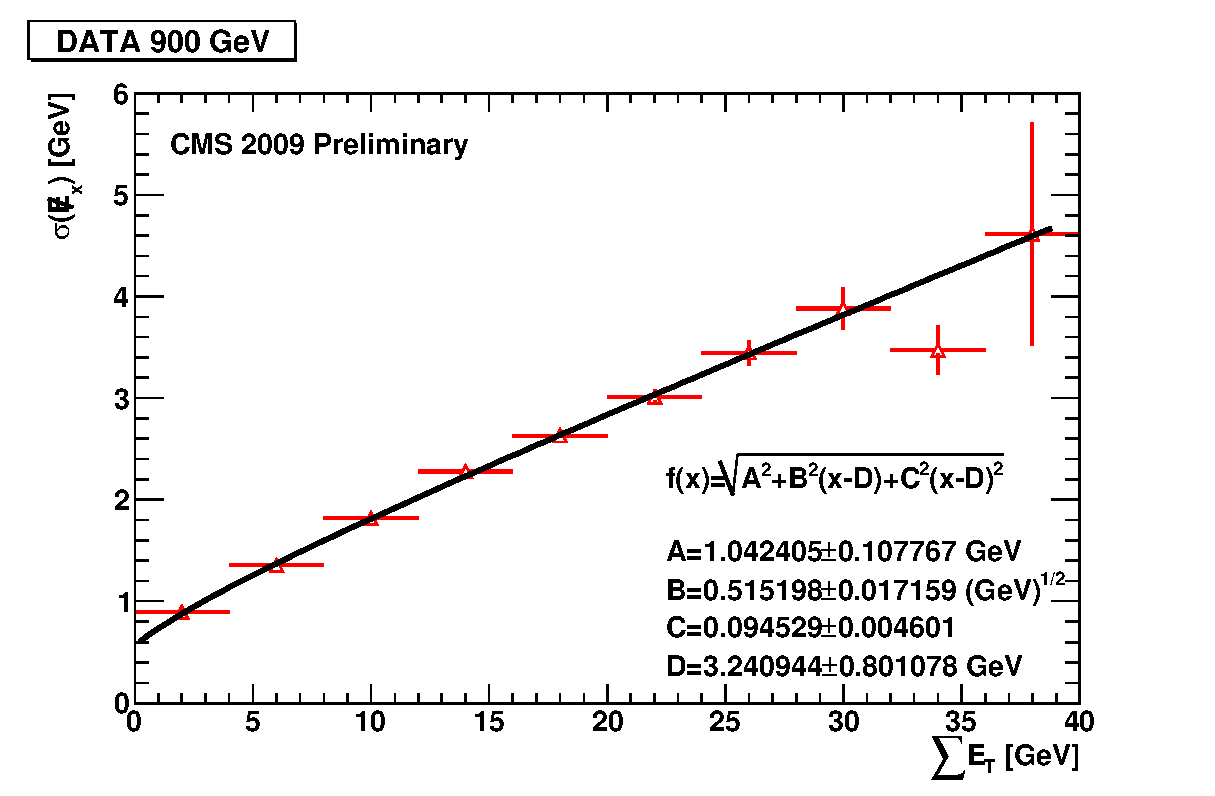
\includegraphics[width=0.5\textwidth]{plots_DataVsMC_MB_900GeV/final_metxsigma_sumet_DATA_900.eps} &
  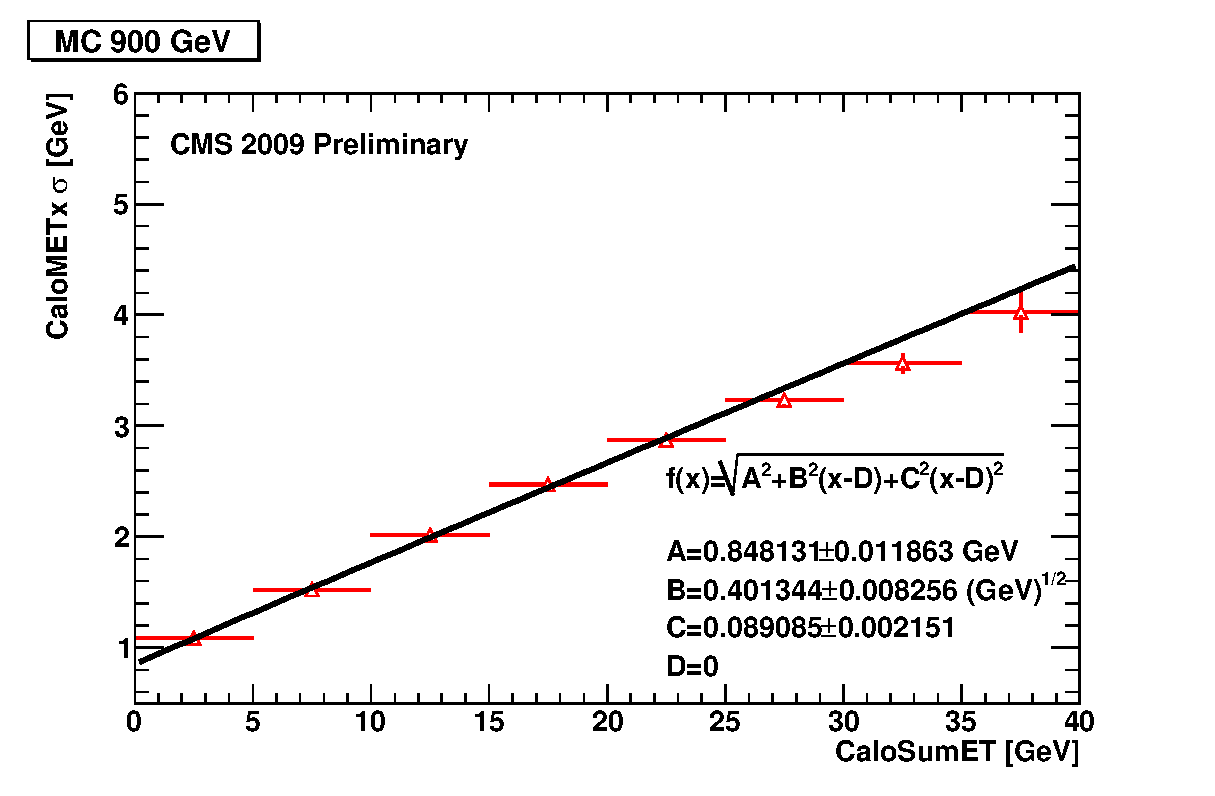
\includegraphics[width=0.5\textwidth]{plots_DataVsMC_MB_900GeV/final_metxsigma_sumet_MC_900.eps} \\
 \end{tabular}
 \caption{\small Fit of the $\sigma\left(\exmiss\right)$ vs. $\sum E_\text{T}$ for data and Monte Carlo at $900$ GeV.\label{fig:MExSigma_vs_SumET_900_fit}}
\end{figure}

\begin{figure}[h!]
 \centering
 \begin{tabular}{ll}
  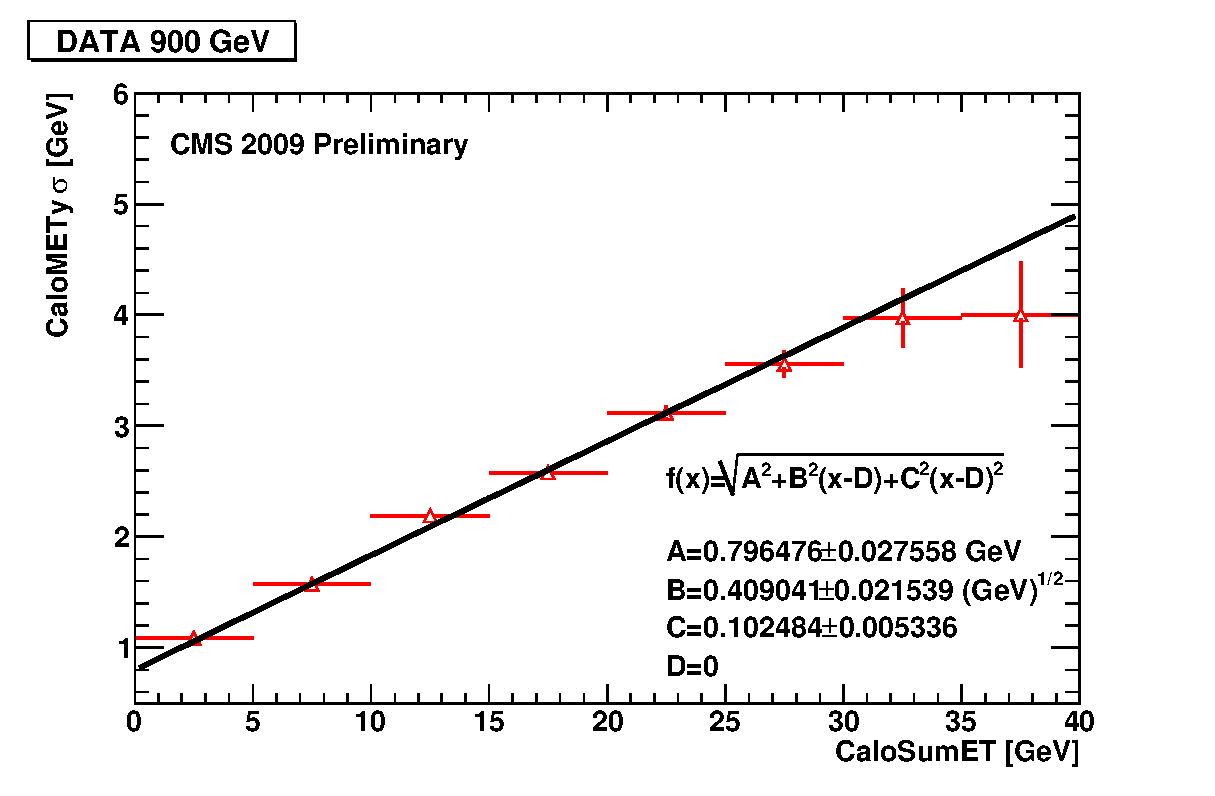
\includegraphics[width=0.5\textwidth]{plots_DataVsMC_MB_900GeV/final_metysigma_sumet_DATA_900.eps} &
  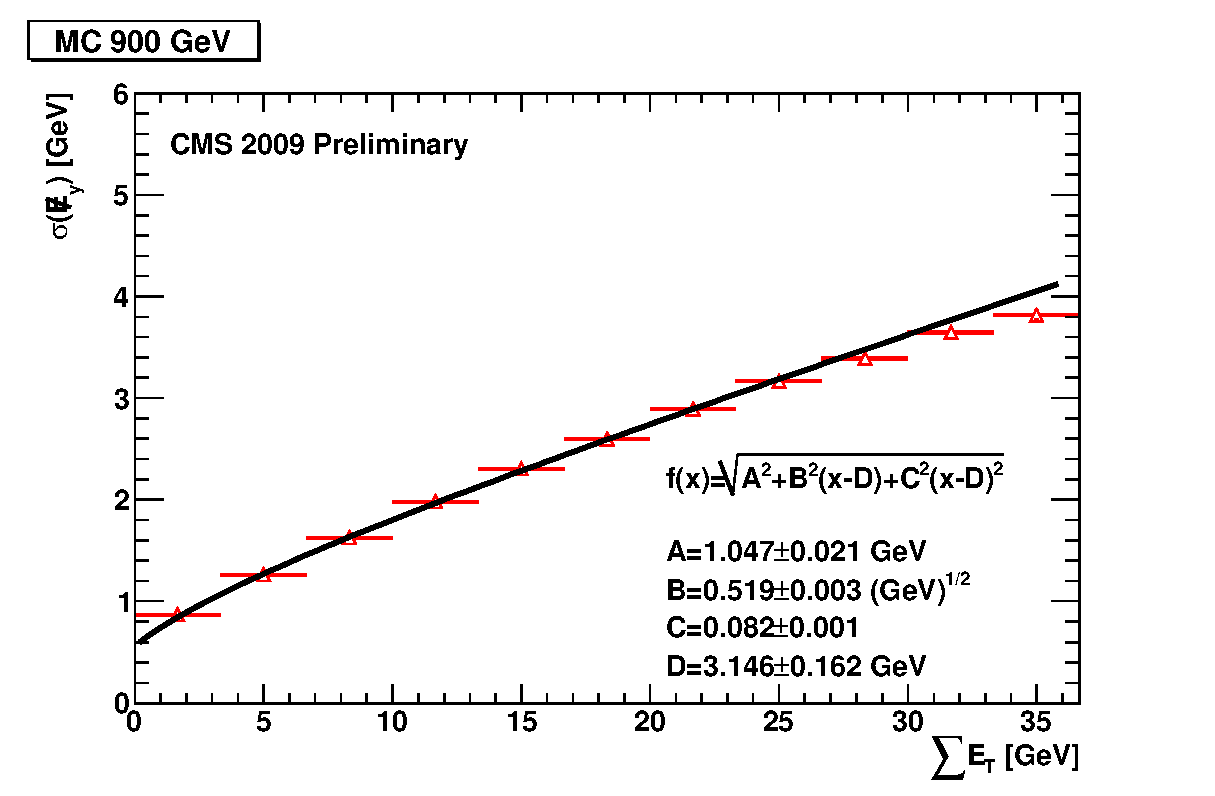
\includegraphics[width=0.5\textwidth]{plots_DataVsMC_MB_900GeV/final_metysigma_sumet_MC_900.eps} \\
 \end{tabular}
 \caption{\small Fit of the $\sigma\left(\eymiss\right)$ vs. $\sum E_\text{T}$ for data and Monte Carlo at $900$ GeV.\label{fig:MEySigma_vs_SumET_900_fit}}
\end{figure}


\clearpage

\subsection{$\etmiss$ and SumET dependence on $\eta$} \label{sec:MetVarVsIeta_900}

The study of $\etmiss$-related quantities in different $\eta$
slices of the combined ECAL+HCAL calorimeter system 
is useful to understand if discrepancies between data and MC 
come from specific regions of the detector.
The plots presented in this section show Mean and RMS values 
of several $\etmiss$-related distributions in different 
$\eta$ rings, i.e. obtained by summing together 
transverse energy of calotowers with the same 
$\eta$ index value and different $\phi$ index values.
Results presented here refers to the 900 GeV data, while results for 2360 GeV
are presented in the Section~\ref{sec:MetVarVsIeta_2360}.

For reference, values of $|i_{\eta}|\le17$, $17<|i_{\eta}|<29$, and $29\le|i_{\eta}|\le41$ 
correspond, respectively, to barrel (EB and HB), endcaps (EE and HE), and forward 
calorimeter (HF), with a few exceptions at the boundaries 
(for example, tower with $i_{\eta}=29$ is shared between both HE and HF).

Figure~\ref{fig:SumET_MeanRMS_vs_ieta_900} shows the Mean and RMS value of 
SumET distribution as a function of $\eta$ ring index for both data and MC at 900 GeV.
\begin{itemize}
\item The Mean and RMS of SumET distribution is in good agreement between 
data and MC for $\eta$ rings in HF, with the exception 
of the ring at $i_{\eta}=41$ (i.e. $\eta=5$), where the average SumET expected from Monte Carlo 
in about twice of what is measured in the data.
A comparison with the noise only distribution 
in Figure~\ref{fig:SumET_MeanRMS_vs_ieta_ZB} shows that, in MinBias events, 
most the transverse energy reconstructed in HF is indeed coming from collisions, and the contribution
from electronic noise is almost negligible.
\item In the positive side of endcap the agreement is also reasonably good 
(at least in the trend as a function of $i_{\eta}$), even if worse than in HF, 
but some larger discrepances are observed in the minus endcap side.
In addition an asymmetry between plus and minus side is observed both in data and simulation.
A direct comparison with Figure~\ref{fig:SumET_MeanRMS_vs_ieta_ZB} shows that the asymmetry 
is also present in noise-only events. This seems to indicate that the transverse energy reconstructed in the 
endcaps still receives a relevant contribution for fluctuations of electronic noise. 
\item In the barrel we observe a good agreement in the approximate range $6<|i_{\eta}|<17$, 
but discrepancies are seen in the very central region. 
The comparison with Figure~\ref{fig:SumET_MeanRMS_vs_ieta_ZB}
show that the amount of transverse energy reconstructed in the barrel for collision 
events is very similar to the one reconstructed in noise only events. 
Therefore, the disageement between data and MC seen for $|i_{\eta}|<6$
is the additional indication of discrepancies between data and MC in 
the barrel noise simulation (in particular this is visible in the $\sumet$ distribution 
for the HB noise simulation, as already noticed in Section~\ref{sc:CaloNoise}).
The fact that the discrepancy is larger in the central region should be due to 
the presence of an $E_{T}$ threshold when forming and summing calotower energy, 
which amplifies the disagreement at low $\eta$ values. 
\end{itemize}

Figure~\ref{fig:MET_MeanRMS_vs_ieta_900},~\ref{fig:METx_MeanRMS_vs_ieta_900}
, and ~\ref{fig:METy_MeanRMS_vs_ieta_900} shows the Mean and RMS value of, respectively,
$\etmiss$, $\exmiss$, and $\eymiss$ distributions as a function of $\eta$ ring 
index for both data and MC at 900 GeV.
Considerations similar to the ones discussed above can also be applied to these plots.
In addition some features are seen in the Mean values of $\exmiss$ and $\eymiss$ distributions
(i.e. not flat at zero for all the $i\eta$ rings), whose trend seems to be reproduced by the MC.
Anyway, the largest shifts from zero are at the level of only 50 MeV, in both x and y component of the $\etmiss$.

\begin{figure}[h!]
 \centering
 \begin{tabular}{ll}
  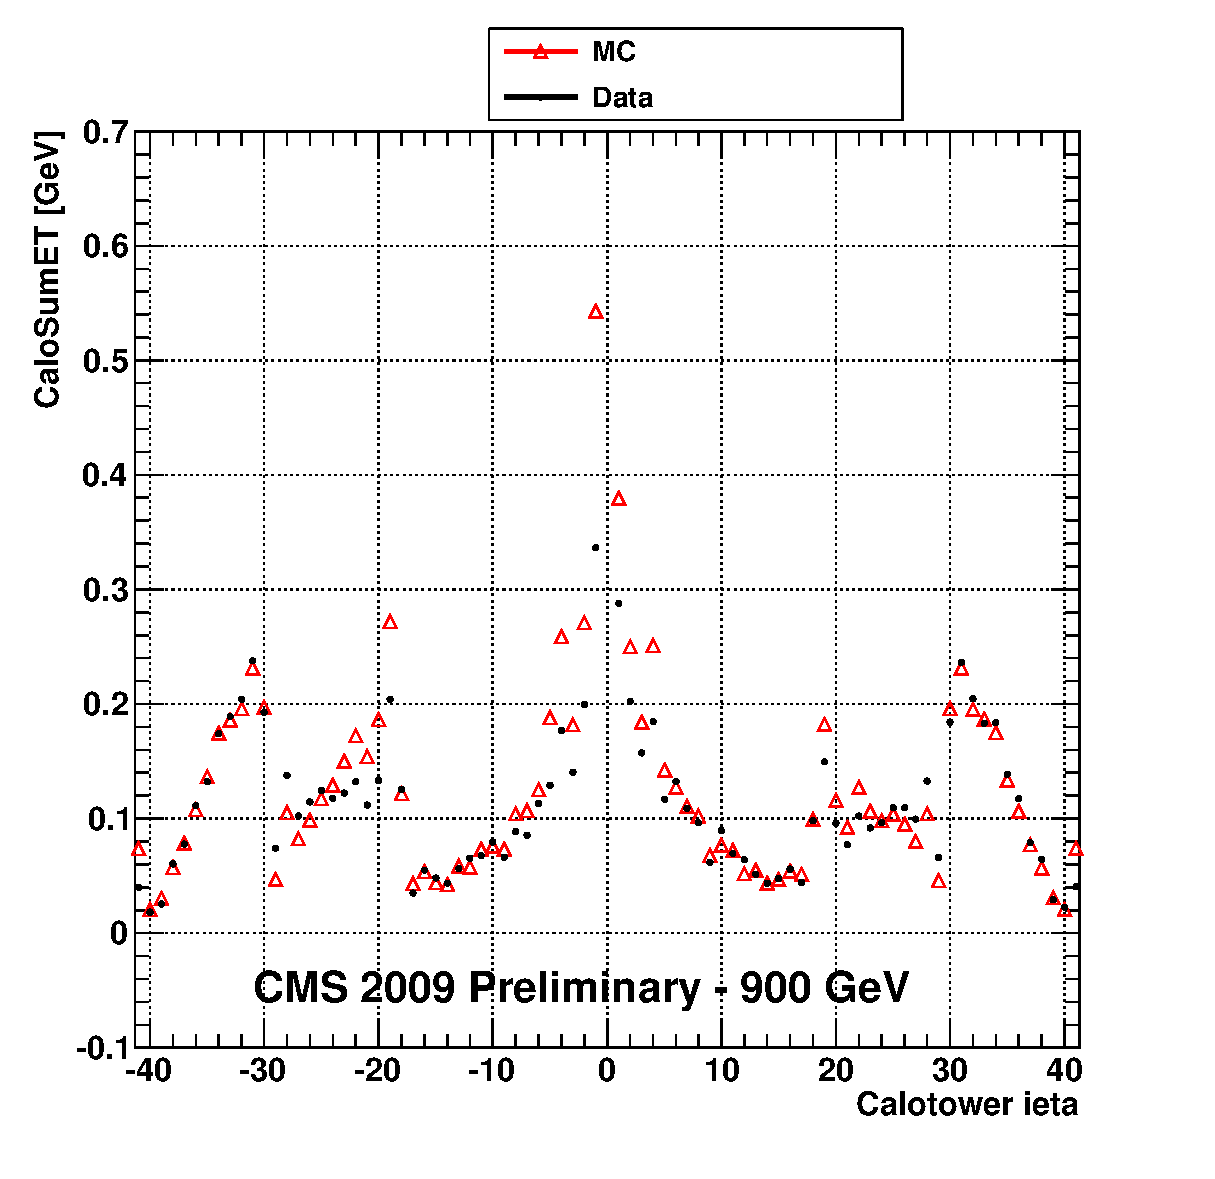
\includegraphics[width=0.5\textwidth]{plots_DataVsMC_MB_900GeV/g_caloSumetMean_vs_ieta_900.eps} &
  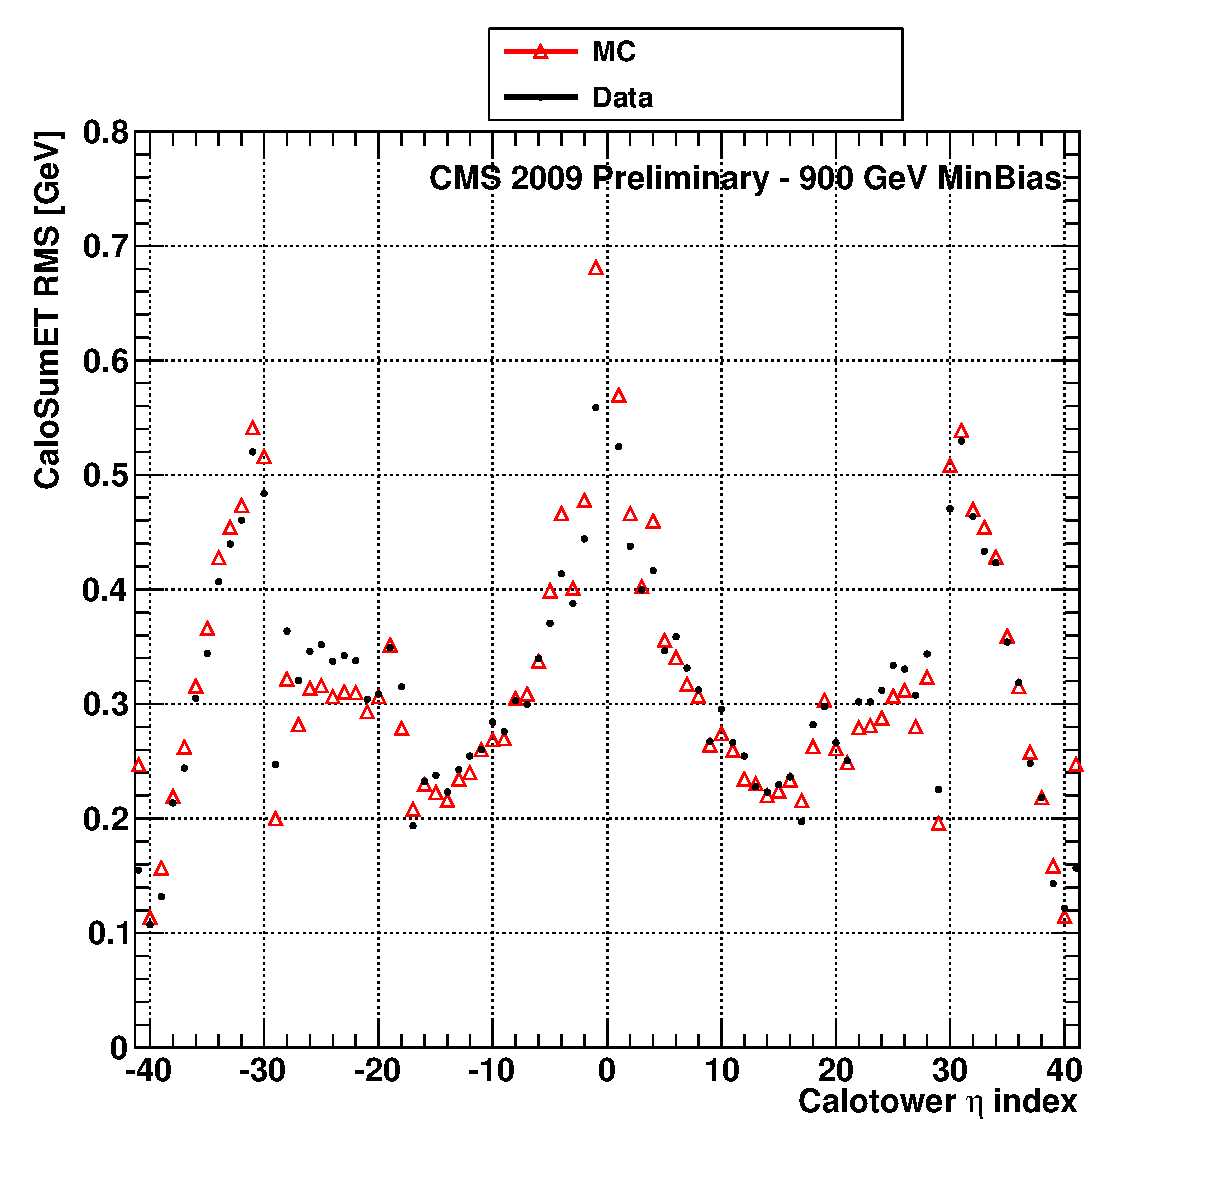
\includegraphics[width=0.5\textwidth]{plots_DataVsMC_MB_900GeV/g_caloSumetRMS_vs_ieta_900.eps} \\
 \end{tabular}
 \caption{\small Comparison of the SumET Mean vs. i$\eta$ of calotowers and SumET RMS vs. i$\eta$ of calotowers between 
          Monte Carlo and data at $900$ GeV.\label{fig:SumET_MeanRMS_vs_ieta_900}}
\end{figure}

\begin{figure}[h!]
 \centering
 \begin{tabular}{ll}
  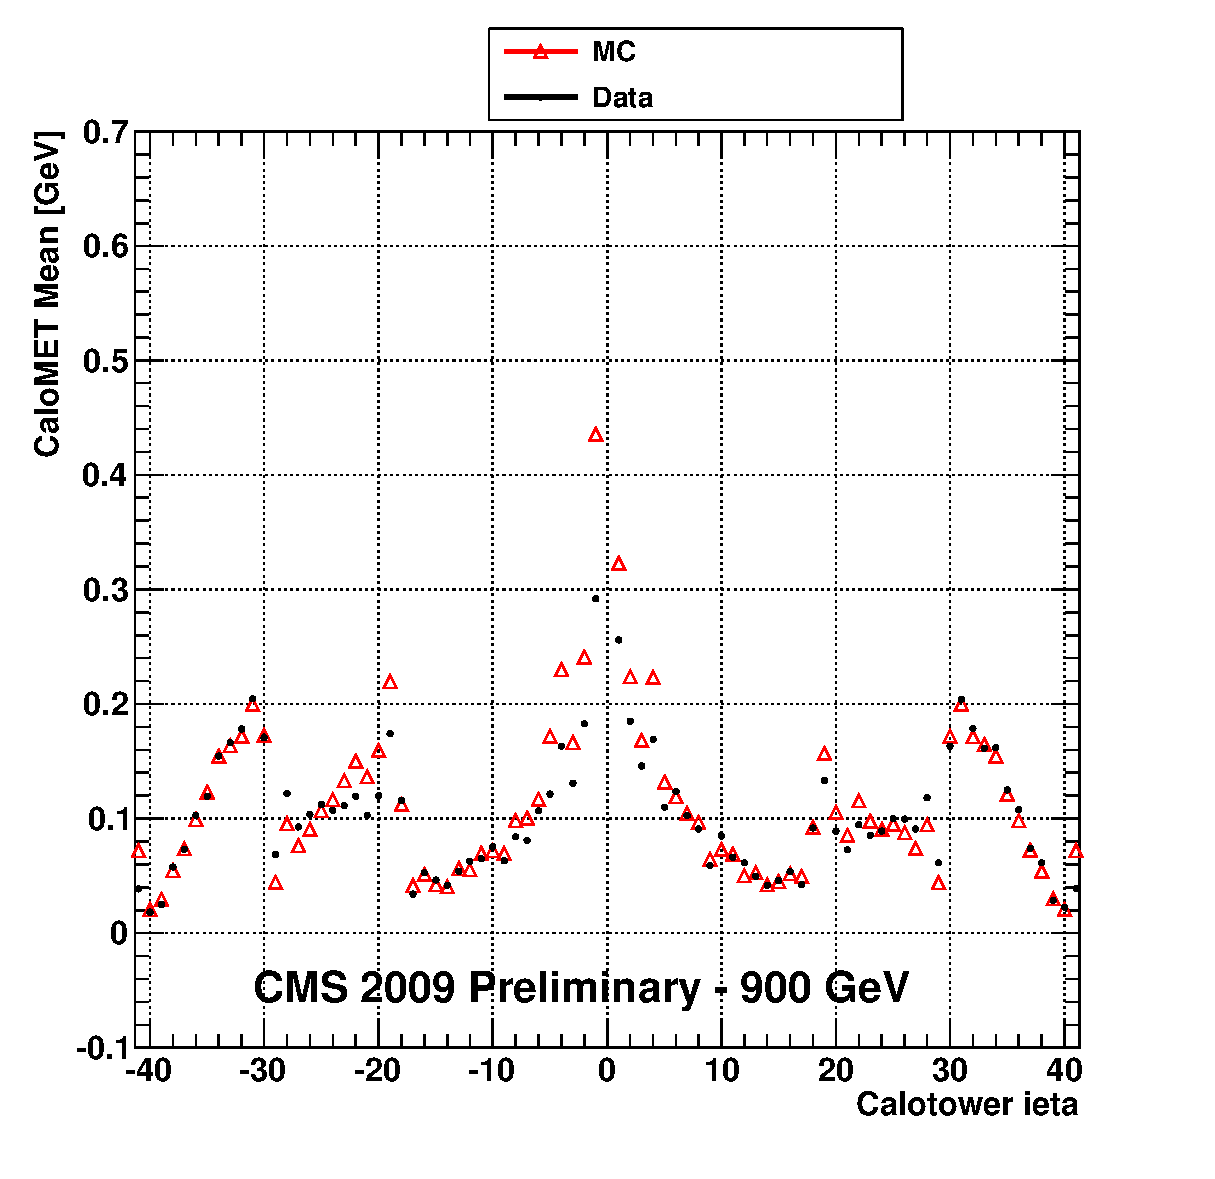
\includegraphics[width=0.5\textwidth]{plots_DataVsMC_MB_900GeV/g_calometPtMean_vs_ieta_900.eps} &
  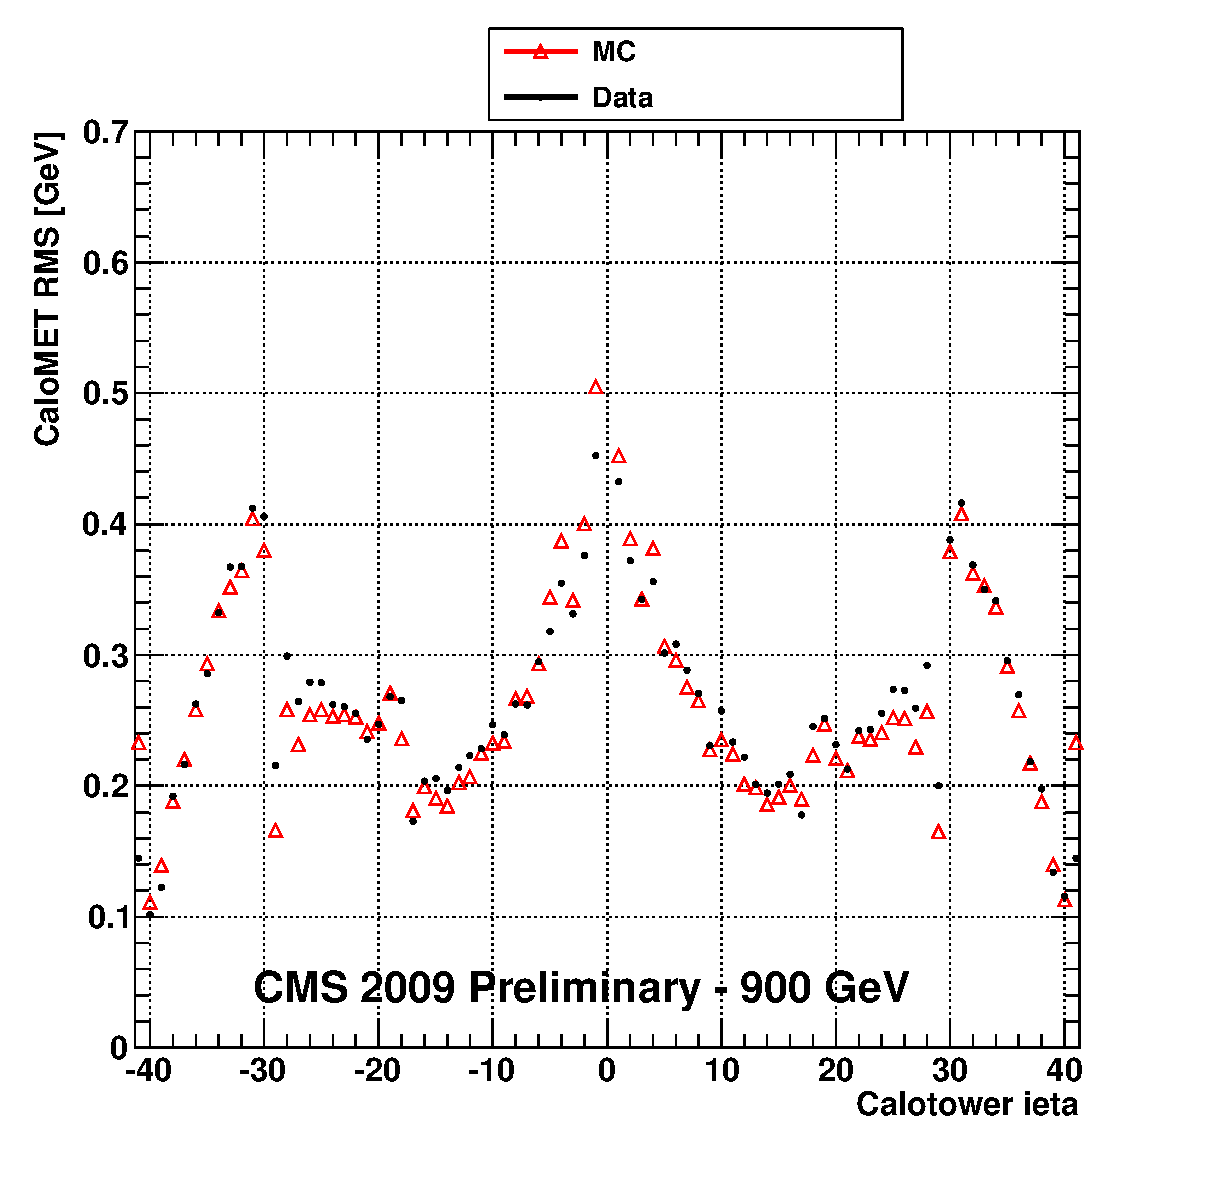
\includegraphics[width=0.5\textwidth]{plots_DataVsMC_MB_900GeV/g_calometPtRMS_vs_ieta_900.eps} \\
 \end{tabular}
 \caption{\small Comparison of the $\etmiss$ Mean vs. i$\eta$ of calotowers and $\etmiss$ RMS vs. i$\eta$ of calotowers between 
          Monte Carlo and data at $900$ GeV.\label{fig:MET_MeanRMS_vs_ieta_900}}
\end{figure}

\begin{figure}[h!]
 \centering
 \begin{tabular}{ll}
  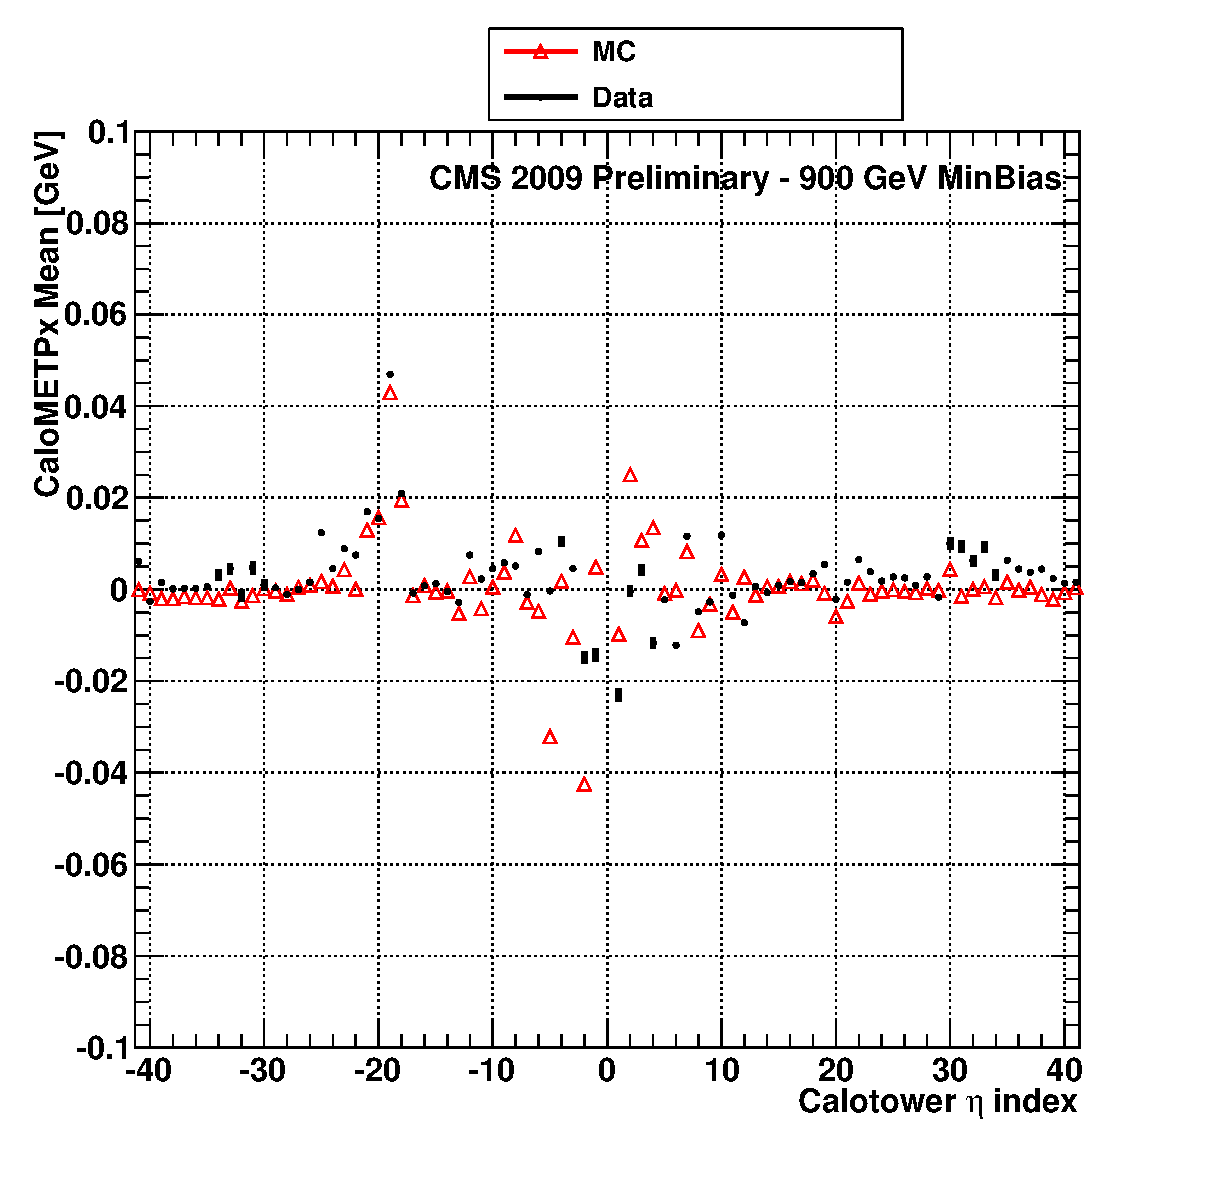
\includegraphics[width=0.5\textwidth]{plots_DataVsMC_MB_900GeV/g_calometPxMean_vs_ieta_900.eps} &
  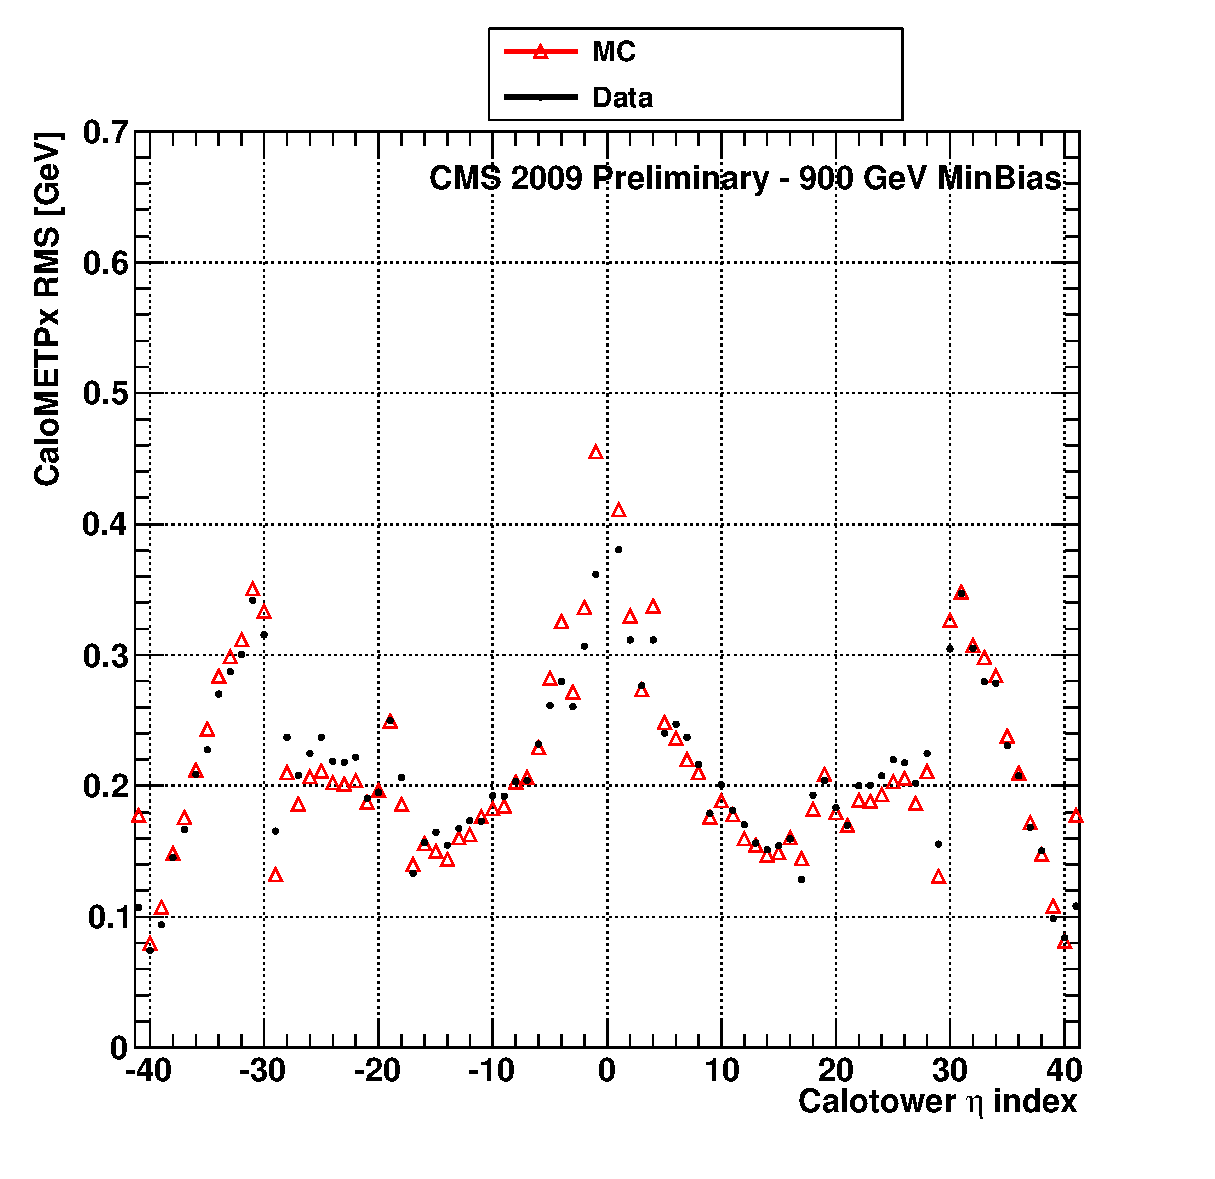
\includegraphics[width=0.5\textwidth]{plots_DataVsMC_MB_900GeV/g_calometPxRMS_vs_ieta_900.eps} \\
 \end{tabular}
 \caption{\small Comparison of the $\exmiss$ Mean vs. i$\eta$ of calotowers and $\exmiss$ RMS vs. i$\eta$ of calotowers between 
          Monte Carlo and data at $900$ GeV.\label{fig:METx_MeanRMS_vs_ieta_900}}
\end{figure}

\begin{figure}[h!]
 \centering
 \begin{tabular}{ll}
  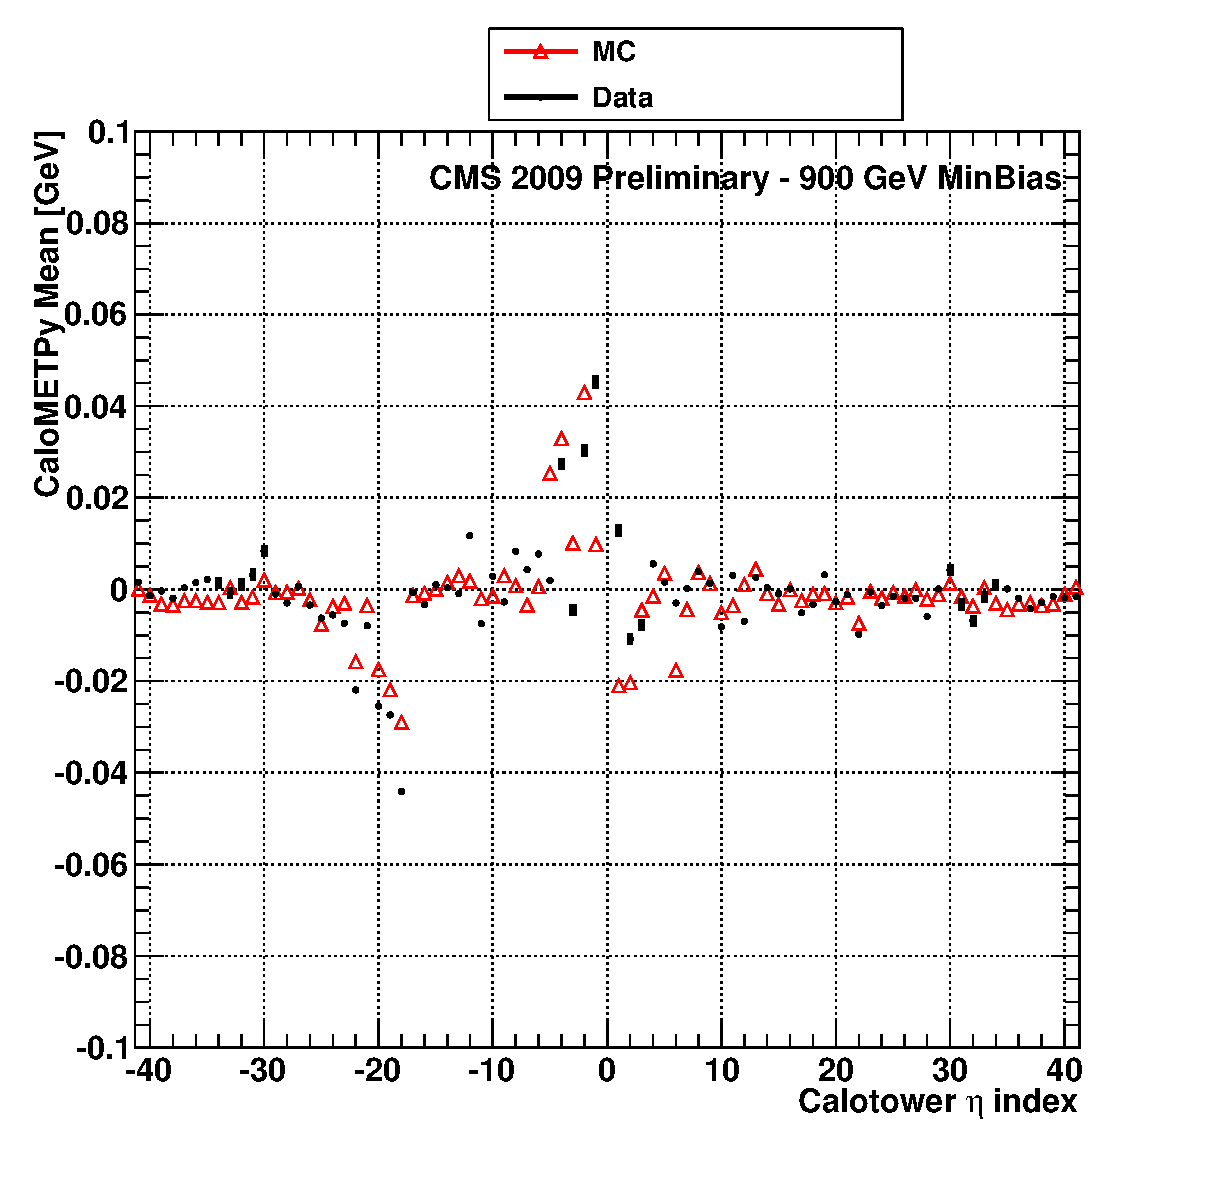
\includegraphics[width=0.5\textwidth]{plots_DataVsMC_MB_900GeV/g_calometPyMean_vs_ieta_900.eps} &
  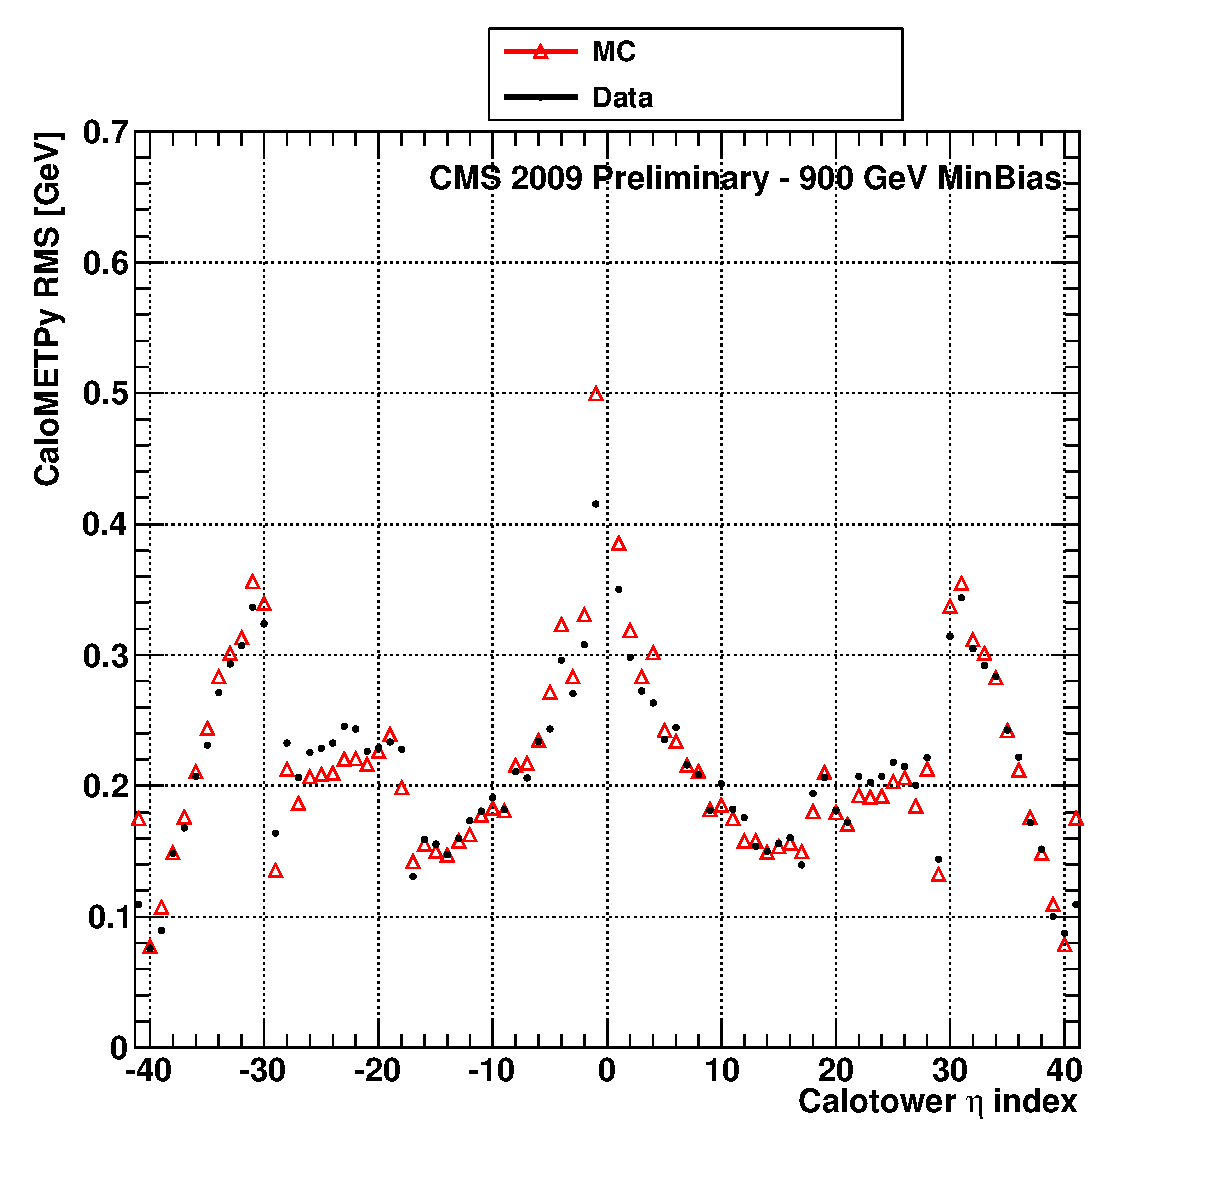
\includegraphics[width=0.5\textwidth]{plots_DataVsMC_MB_900GeV/g_calometPyRMS_vs_ieta_900.eps} \\
 \end{tabular}
 \caption{\small Comparison of the $\eymiss$ Mean vs. i$\eta$ of calotowers and $\eymiss$ RMS vs. i$\eta$ of calotowers between 
          Monte Carlo and data at $900$ GeV.\label{fig:METy_MeanRMS_vs_ieta_900}}
\end{figure}

\clearpage
